\chapter{Design}
\label{chap:design}
This chapter describes the internal wiring of the application and the reasons that lead to this design.
First, it explains the technology used: the programming language, frameworks and most relevant libraries.
Next, it presents the architecture of the system and the application, the software patterns and sequence diagrams of the most relevant operations.
Finally, it includes a physical view with deployment diagrams.

Reverse engineering the current project involves 3 activities related to technology and implementation details: \textbf{code restructuring}, \textbf{data restructuring} and\textbf{ forward engineering}.
No modifications in the code of the old version of Flango \cm are scheduled: there is no code or data restructuring.
However, there are some adaptations to be done in the \flangobe (\ac{API}), \ac{XML} and robotBehaviour:

\paragraph{Changes in \flangobe} The \ac{API} is designed to return \ac{XML} in all cases.
Most of the time this is desirable (e.g. requests to get screens) but in cases where normal exchange of information is done between the two systems, \ac{JSON} is a better option for the new technology.
It is less verbose (minimise bandwidth) and has a straight-forward translation to JavaScript objects.

\paragraph{Changes in \ac{XML}} The \ac{XML} syntax is designed to work isolated.
The new version, however, can mix \ac{XML} with \ac{HTML} thanks to Angular.
Some tags of the \ac{XML} vocabulary conflict with \ac{HTML}. For instance, \texttt{caption}. Solution: add a namespace \texttt{fl} to all tags. 
Therefore, in the new version a \lstinline$<ui type="base-button"></ui>$ becomes \\ \lstinline$<fl:ui fl:type="base-button"></fl:ui>$ .

\paragraph{Changes in robotBehaviour} Current interoperation between Flango \cm and the robot is limited to robotBehaviour.
This communication is done with JavaScript callbacks and \acp{URL}.
To decouple the \cm as much as possible from the rest of the robot, the new system uses \ac{ROS} Topics and ROS Bridge

\paragraph{Forward Engineering} A program that depends on a dead browser plug-in with performance issues is not sustainable.
A solution is completely  redesigning, recoding and retesting the program, even with a different technology that makes it more flexible, open to new developers and without performance problems.

\section{Technology}
The project of this thesis, Flango \cm, is designed to work client side in a web browser.
That is, in the robot, as a client, despite the fact that the server is in the robot as well.
The natural technology in this environment is JavaScript, \ac{HTML} and \ac{CSS}.
It uses the Google Angular framework with jQuery.
Angular \textit{teaches the browser new syntax}.
That is, instead of parsing the \ac{DOM} tree and building the \ac{GUI}, it defines the behaviour of new tags in \ac{HTML} documents that can be treated as regular \ac{HTML} nodes in the \ac{DOM}.
It interoperates with other systems built with a different technology: components in the robot use \ac{ROS} and the \flangobe has an \ac{API} (see sections \ref{sec:context}, \ref{sec:interaction} and \ref{sec:interoperability} on page \pageref{sec:context}).

\subsection{JavaScript}
JavaScript is probably the most misunderstood and at the same time popular language of all times.
It is the language of the web browser and works closely with the \ac{DOM}, the \ac{API} of the browser.

Some good and key ideas in the language include \textbf{functions}, \textbf{loose typing}, \textbf{dynamic objects} and an expressive \textbf{object literal notations}.
On the other side, the programming model is based on global variables (although the language has tools to mitigate this) \cite{Crockford}.
\textbf{Functions are first class objects} and can be passed as arguments or returned from functions, just like any other object.
This allows the language to have function scope and lexical scoping: \\
\textbf{Function scope} means that variables defined in a function are visible in the entire function, an approach different from block scope in languages like C or Java.\\
\textbf{Lexical scoping} defines how names are resolved in nested functions: the scope of an inner function contains the scope of the parent function, even if the parent has returned.
This scoping is key in the strategy to read and inherit properties with the \ac{XML} that defines UI Components.

JavaScript is an \textbf{object-oriented prototype-based language}, not a class-based language.
It has a class-free object system in which objects inherit properties directly from other objects.
Behaviour reuse (inheritance) is achieved by cloning existing objects (the prototypes).
Crockford explains the prototypal inheritance mechanism \cite{Crockford:proto}:
\begin{quote}
So instead of creating classes, you make prototype objects, and then use the object function to make new instances. Objects are mutable in JavaScript, so we can augment the new instances, giving them new fields and methods. These can then act as prototypes for even newer objects. We do not need classes to make lots of similar objects.
\end{quote}

\subsection{AngularJS}
\paragraph{Overview} Angular is a \ac{MVC} framework for dynamic web applications that enforces a strict separation of concerns.
\ac{HTML} was created to declare static documents and needs libraries and frameworks to enable application development.
Angular lets developers use \ac{HTML} in the templates and extend the language syntax to express reusable components.
It \textit{teaches the browser new syntax} through a construct called Directive.
Features:
\begin{itemize}
    \item Tools to build \ac{CRUD} Applications: data-binding, basic templating directives, form validation, routing, deep-linking, reusable components, dependency injection.
    \item Tools to test: unit-testing, end-to-end testing, mocks.
\end{itemize}

Flango \cm reads \ac{XML} and renders it as \ac{HTML}.
There are two possible approaches: parsing the \ac{DOM} tree in the browser or teaching the browser new syntax.
This project uses the latter: instead of developing an algorithm to traverse the tree and render elements, it defines reusable components (Angular Directives) and includes the \ac{XML} files in the appropriate places in the \ac{DOM}. 
The browser already traverses the tree in order to display the page and there is no need to do it manually.
Normally a browser ignores an element that does not belong to the \ac{HTML} specification (e.g. \lstinline$<fl:ui fl:type="base-button"></fl:ui>$)
With Angular, the browser runs the behaviour defined in the reusable component.

\paragraph{Building Blocks} There are several key components in Angular to build the application.

\begin{description}
    \item[Controller] A function that binds the view with the model. It typically assigns objects to the \$scope variable to expose them to the template.
    \item[Directive] A construct to extend HTML with custom attributes and elements. It defines the template of the reusable component, the behaviour, the attributes, etc. For instance, the directive \texttt{flBaseButton} states that the node \lstinline$<fl:ui fl:type="base-button">$ in the \ac{DOM} tree should be transformed into a simple \texttt{button} using the theme template \texttt{baseButton.xml}. 
    \item[Service] Singleton that encapsulates reusable business logic independent of views. For instance, a service to handle the configuration of the application. They can be injected in controllers, directives or other services.
    \item[Filter] A function that formats the value of an expression for display to the user. For instance, a filter to display a Number with currency format.
    \item[Module] These building blocks are grouped in Modules. They can have dependencies between them.
\end{description}

The framework provides all the necessary tools to use unit and \ac{E2E} testing from the very beginning of the project. 
\Fref{chap:testing} explains them in depth.
    
\paragraph{Compile-Link} To make directives possible Angular has a compiler.
In this context, compiling means attaching event listeners to the \ac{HTML} to make it interactive.
The compiler traverses the \ac{DOM} tree in two phases:
Firstly it looks for tags that have directives associated (e.g. \lstinline$<fl:ui fl:type="base-button">$ or even native \ac{HTML} elements \lstinline$<a>$).
Secondly it binds the model to the view.
The compiler allows developers to attach behaviour to any \ac{HTML} element or attribute and even create new HTML elements or attributes with custom behaviour.
Angular calls these behaviour extensions directives.

Listings \ref{design-order-of-exec-1} and \ref{design-order-of-exec-2} illustrate the order of execution.

\lstinputlisting[label=design-order-of-exec-1,language=xml, caption={Order of execution of directives}]{src/example-order-directives.xml}

\lstinputlisting[label=design-order-of-exec-2,language=bash, caption={Result of execution of directives}]{src/result-order-directives.text}

The role of these functions is:
\begin{itemize}
\item \textbf{Directive Controller}: similar to regular controllers but accessible from other directives. 
\item \textbf{Compile} finds new directives and runs their compile function. Modifications to the \ac{DOM} before applying the template can be done here.
\item \textbf{Link}: binds data to the view. Modifications to the final \ac{DOM} are safe to do here.
\end{itemize}

\paragraph{Directive} At a high level, directives are markers on a \ac{DOM} element (such as an attribute, element name, \ac{CSS} class or a comment) that tell Angular's \ac{HTML} compiler to attach a specified behaviour to it or even replace it with another element.
The \ac{HTML} compiler finds elements that match directives. 
For example, for \lstinline$<div ng-controller="myCtrl">$, the element \texttt{div} matches the directive \texttt{ngController}.
An example in Flango \cm : when the browser finds \lstinline$<fl:width>150</fl:width>$ in the \ac{DOM}, the element \texttt{width} matches the directive \texttt{flWidth}.
The \texttt{flWidth} directive is restricted to elements (it matches \lstinline$<fl:width>150</fl:width>$ but not \lstinline$<div fl:width>150</div>$ because it is an attribute), and it has a custom \texttt{link} function that performs some computation.

    
\subsection{HTML5}
FIXME maybe not useful. maybe just html

\subsection{SASS}
Writing plain \ac{CSS} can be tedious and error-prone.
SASS stands for Syntactically Awesome \ac{CSS} and is a pre-processor with syntax advancements that add features to \ac{CSS}.
SASS is an extension of \ac{CSS3}, adding nested rules, variables, mixins, selector inheritance, and more.
SASS code is translated into well-formated, standard \ac{CSS} using the command line tool.
This makes reusing and extending \ac{CSS} easier.
SASS has two syntaxes.
This project uses the newest, known as \ac{SCSS} (Sassy CSS).

A key feature in this project is the \lstinline$@extend$ directive: it tells \ac{SASS} that one selector should inherit styles of another selector.
Example: the style \texttt{base-button} has a grey background. The style \texttt{button} sets the size of the element to $100 x 50 px$.
Because all \texttt{base-button}s are \texttt{button}s, the first should inherit the style from the second instead of replicating it, like one would do with \ac{OOD}.
With \ac{HTML} this would be written \lstinline$<div class="base-button button" />$.
With SASS one can write \lstinline$.base-button { @extend .button }$ and keep \ac{HTML} cleaner: \\ \lstinline$<div class="base-button" />$ instead of \lstinline$<div class="base-button button" />$

SASS variables and mixins make it easier to create themes for Flango \cm and provide a way to ensure visual consistency (e.g. all themes can have palettes of the same size).

\subsection{Robot Web Tools}
Robot Web Tools is a collection of open-source modules and tools for building web-based robot applications.
It provides 3 core libraries to communicate with \ac{ROS} on the robot over rosbridge's WebSocket server: roslibjs, ros2js, and ros3djs.
This project uses roslibjs\footnote{\url{https://github.com/RobotWebTools/roslibjs}} to subscribe and publish to \ac{ROS} Topics.

\section{Architecture}
This section contains details about the architecture of the system (ROS) and the project of this thesis (Flango \cm ). 
Flango \cm is a piece in \ac{ROS}, which is similar to a \ac{SOA} system, and interoperates with it using its message system.
The following pages have a high-level description of the system architecture and the patterns used.

\subsection{Robot Operating System}
The operating system of \reem{H} is Ubuntu Linux. \acf{ROS} is a framework for robot software development that provides operating system-like functionality on a heterogeneous computer cluster.
It was originally developed in 2007 as part of the Stanford AI Robot (STAIR) project to create an architectural framework for modular, tool-based development of robotic software.
It has a loosely coupled architecture with nodes, messages, topics and services, similar to \ac{SOA} \cite{ROS:2009}.

Nodes are processes that perform computation, a "software module". 
Nodes communicate with each other by publishing/subscribing with two protocols:
\begin{description}
\item[Topics] asynchronous. message passing (publish/subscribe). Typed by a \ac{ROS} Message
\item[Services] synchronous. \ac{RPC} (pairs of request/response messages). Typed by a \ac{ROS} Service
\end{description}

Messages are strictly typed data structures. There are some available by default, like \texttt{std\_msgs/String} and other primitive types.
To find a service in this peer-to-peer topology, there is a lookup mechanism: \emph{rosmaster} (see \fref{fig:design-ros-topics} and \fref{fig:design-ros-services}).

The robot has two parts: robotBehaviour and Stacks.
Part of the code of the robot (robotBehaviour) does not follow the \ac{ROS} workflow but still uses Topics to communicate with the Stacks, the part of the project that does use \ac{ROS}.
In Stacks there are Servers and ActionServers that provide Services.

Flango \cm is a component in this system that communicates with robotBehaviour using \ac{ROS} Topics and two types of messages.
It is not designed strictly as a service to handle synchronous requests but it is able to use Topics to have asynchronous requests and provide feedback, like ActionServers.
A typical use of a \ac{ROS} Topic is setting the language of the \cm or sending an action to robotBehaviour (e.g. shake hands, say a sentence).
robotBehaviour is not a \ac{ROS} service and therefore it can not handle request/responses like other components in the system.
Topics are the only way to communicate with it.

\begin{figure}[htb]
    \centering
    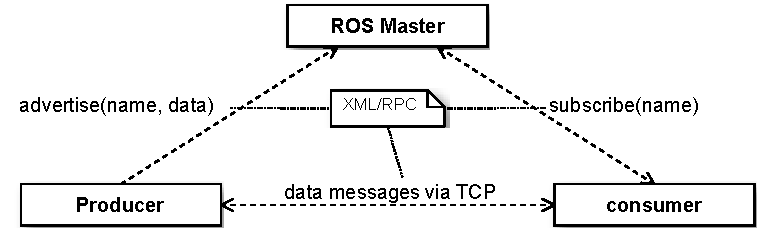
\includegraphics{figures/design/ros-architecture-topics.pdf}
    \caption{High-level view of the ROS Architecture (Topics)}
    \label{fig:design-ros-topics}
\end{figure}

\begin{figure}[htb]
    \centering
    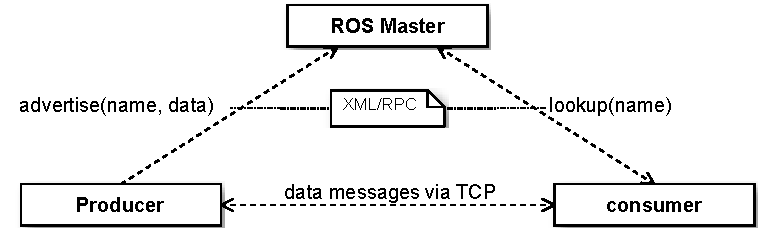
\includegraphics{figures/design/ros-architecture-services.pdf}
    \caption{High-level view of the ROS Architecture (Services)}
    \label{fig:design-ros-services}
\end{figure}

\subsection{\acf{MVC}}
\acf{MVC} is a decoupled architecture with a strong separation of responsibilities (\fref{fig:mvc-overview}).
\begin{description}
    \item[Model] (application state). Maintains application state and notifies dependent views and controllers when changes occur (with the observer pattern)
    \item[View] (output) queries the model to print [parts of] it, listens for changes in the model
    \item[Controller] (input) Listens for input and tells the model or the view to change accordingly
\end{description}

It is possible to have multiple views and controllers for the same model and they can be reused for other models.

Angular applications take the most of the framework when they are designed with a \ac{MVC} architecture.
A typical use case in a \ac{MVC} application might be:
\begin{itemize}
    \item Model: \texttt{[orange, apple, pineapple, coconut]}
    \item View: displays a list of 2 random pieces of fruit
    \item Controller: logic to fetch two pieces of fruit
\end{itemize}

Flango \cm does not have a \ac{GUI} or a set of predefined and stable use cases: this changes for every content application.
The system only knows the use cases after loading the content application.
There can not be controllers for application-specific use cases and the view is created dynamically from the model.

\begin{itemize}
    \item \textbf{Model}: screens definitions, entities, configuration... stored in the backend
    \item \textbf{View}: built dynamically from the model. The application loads screens as the user navigates to \ac{URL}s and transforms them to \ac{HTML} so that they can be displayed in the browser.
    \item \textbf{Controller}: Typically, controllers in Angular manage the \texttt{\$scope} and expose behaviour to the View. This application has some generic (as opposed to application-specific) ones. For example: an instance of \texttt{ActionCtrl} for each button, a \texttt{ROSBridgeCtrl} to respond to requests from ROS Bridge, etc. Directives also have a special type of controllers: Directive Controllers are defined within the context of one directive but they can be injected into other directives to facilitate inter-directive communication. For example, a controller in the \texttt{flUi} directive manages its properties (\texttt{x}, \texttt{y}, \texttt{width}, \texttt{height}, \texttt{caption}...). \texttt{flWidth}, \texttt{flX}, and other directives use the controller in \texttt{flUi}.
\end{itemize}

Angular uses an \ac{MVC} pattern with two-way data binding \fref{fig:mvc-with-observer}: changes in the view are reflected to the model immediately and viceversa in order to use the model as a single source of truth.
Controllers use the \texttt{\$scope} to expose values and behaviour to the view: they update the object that is used in the view.
The \texttt{scope} is an object that refers to the application model.
FIXME LANGUAGE Informally, it is the glue between the controller and the view.
FIXME: SURE? Controllers are completely separated from the view and unaware of it: they just expose values but do not manipulate the \ac{DOM} or read it in any way to make testing easier.

\begin{figure}[htb]
    \centering
    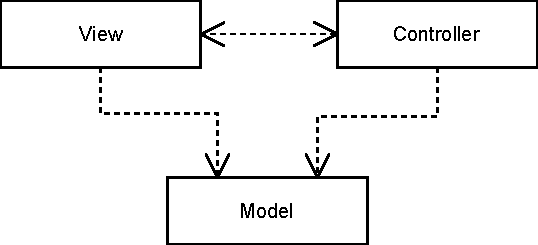
\includegraphics{figures/design-patterns-mvc-1.pdf}
    \caption{\ac{MVC} overview}
    \label{fig:mvc-overview}
\end{figure}

\begin{figure}[htb]
    \centering
    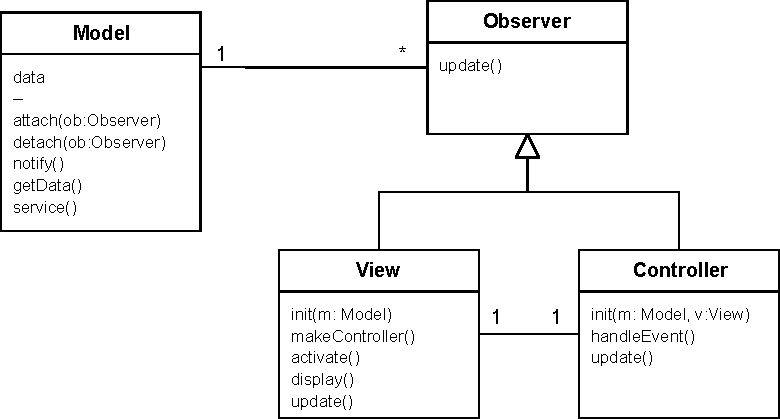
\includegraphics{figures/design-patterns-mvc-2.pdf}
    \caption{\ac{MVC} with observer pattern}
    \label{fig:mvc-with-observer}
\end{figure}

\subsection{Software Patterns}
This subsection is a high-level description of the most relevant software patterns in the project: dependency injection and service locator, factory method, module and revealing module, command and FIXME Remote facade.

\paragraph{Dependency Injection and Service Locator} 
After applying the Creator Pattern (\acs{GRASP} \cite{GoF:1995}) class \texttt{A} creates objects of dependant class \texttt{B}.
One of the \acs{SOLID} principles, dependency inversion, states that one should "Depend upon Abstractions. Do not depend upon concretions."
\textbf{Dependency Injection} is one of the implementations of this principle \cite{Fowler}.

In general there are 3 ways an object can use another one in JavaScript:
\begin{enumerate}
	\item With a \texttt{new} operator (\texttt{A} creates \texttt{B})
	\item Using global variables (\texttt{A} uses a global \texttt{B})
	\item Pass in the dependency to where it is needed
\end{enumerate}

\textbf{Dependency Inversion} means that objects do not create other objects on which they rely to do their work.
They get the dependencies from an outside source (e.g. an \ac{XML} configuration file).
\textbf{Dependency Injection} means that this is done in a transparent way for the object.
The dependency is supplied to the software component.

\begin{figure}[htb]
    \centering
    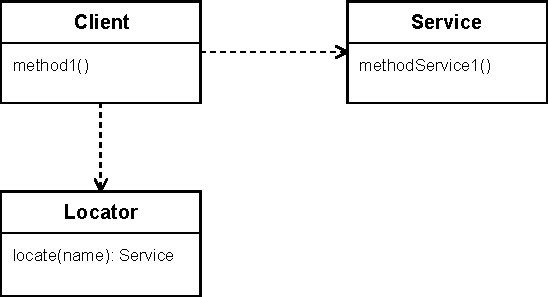
\includegraphics{figures/design-patterns-servicelocator.pdf}
    \caption{Pattern: Service Locator}
    \label{fig:design-service-locator}
\end{figure}

The framework encourages the use of this pattern in all components. 
More specifically, the framework uses a \textbf{Service Locator} (\fref{fig:design-service-locator}) called \texttt{\$injector} that manages the dependency creation.
This allows services to be used in controllers and directives by their name.
The client class does not need to know the concrete implementation of the service. 
With this principle it is easy to mock classes for unit testing and change components in general.


\paragraph{Factory} Directives, controllers, services... are registered on modules. 
The \texttt{module.directive} \ac{API} registers them. 
It takes a normalised name and a factory function (\fref{fig:design-patterns-factory}) that returns an object with the fields that can be exposed to classes that use it.
For example, a Directive Definition Object or a Service.

\begin{figure}[htb]
    \centering
    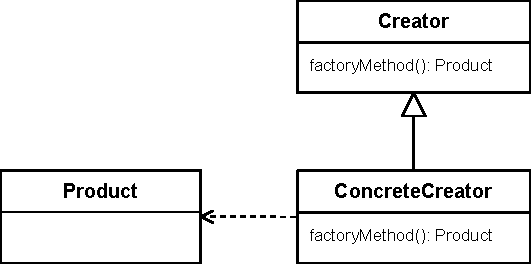
\includegraphics{figures/design-patterns-factory.pdf}
    \caption{Pattern: Factory Method}
    \label{fig:design-patterns-factory}
\end{figure}

\paragraph{Revealing Module} Modules typically help in having separated the units of code for a project.
JavaScript does not support the concept of classes but it does support special constructor functions that work with objects. 
The \texttt{new} keyword used in a call to a constructor function makes JavaScript instantiate the new object with members defined by that function.
Modules are a way to emulate the concept of classes.
There are several options to implement them.
The \textbf{module pattern} encapsulates privacy, state and organisation using closures.
Only a public \ac{API} is returned, keeping everything else hidden within the closure private.
With the \textbf{Revealing Module Pattern} \cite{Osmani:2012} the code of the module is simplified: all variables and functions are defined in the private scope and returns an anonymous object with pointers to the private properties that should be revealed.
An implementation is shown in listing \ref{impl-factory-reveal} on page \pageref{impl-factory-reveal}.

\paragraph{Remote Facade} FIXME: sure? do I have a remote facade in the app, in a controller? rosbridgectrl?

\paragraph{Command} 
Sometimes requests are issued to objects without knowing anything about the operation being requested or the receiver.
The command pattern is a behavioural design pattern in which an object is used to represent all the information needed to call a method at a later time. 
It lets objects make requests of unspecified application objects by turning the request itself into an object.
This object can be stored and passed around like other objects \cite{GoF:1995}.
Other names are \textbf{Transaction} or \textbf{Action Pattern}  

\begin{figure}[htb]
    \centering
    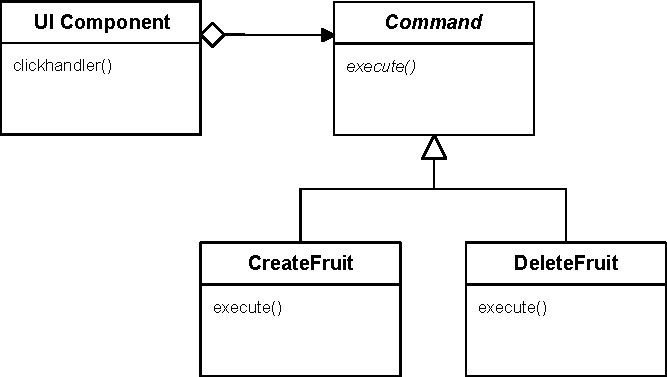
\includegraphics{figures/design-patterns-command-1.pdf}
    \caption{Pattern: Command (general)}
    \label{fig:design-command-general}
\end{figure}

\begin{figure}[htb]
    \centering
    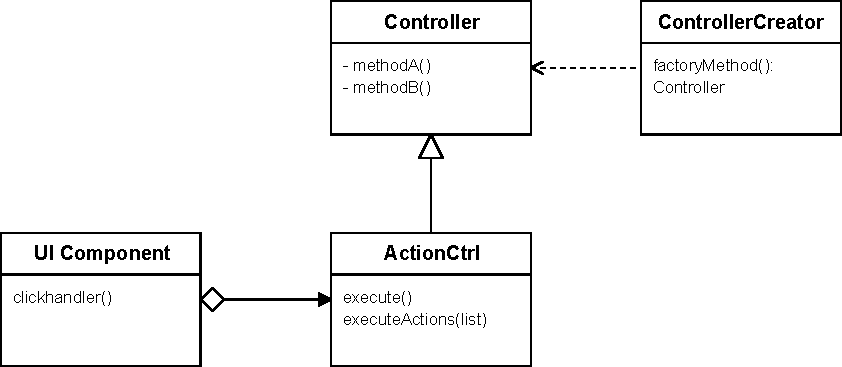
\includegraphics{figures/design-patterns-command-flango.pdf}
    \caption{Pattern: Command (in Flango \cm)}
    \label{fig:design-command-flango}
\end{figure}

\Fref{fig:design-command-general} shows the class diagram of this pattern in the context a traditional object-oriented programming language.
With JavaScript there are no abstract classes.
Osmani \cite{Osmani:2012} proposes having only concrete classes with a common \texttt{execute()} method.
\Fref{sec:controllers} contains a description of the implementation in JavaScript of this pattern.

With a simple controller (\fref{fig:design-command-general}) one would call the methods in the object.
While this is correct, at the time the \ac{GUI} is built the \texttt{UI Component} does not know about the operations being requested.
For example, there is no way to define the behaviour for a \texttt{UI Component::Button} click handler.
Only the content application knows it.
By adding an \texttt{execute} method to \texttt{ActionCtrl}, used in \texttt{UI Components} that accept the tag \texttt{onclick} and \texttt{action}, methods can be called without knowing them (\fref{fig:design-command-flango}).

\subsection{Orientation to Web Components}
Web Components is a set of specifications that let web developers use \ac{HTML}, \ac{CSS} and JavaScript to build widgets that can be reused easily and reliably.
A web component consists of five pieces \cite{W3CComponents:2013}:
\begin{description}
    \item[Templates] define chunks of mark-up that are inert but can be activated for use later.
    \item[Decorators] apply templates based on CSS selectors to affect rich visual and behavioural changes to documents.
    \item[Custom Elements] let authors define their own elements, with new tag names and new script interfaces.
    \item[Shadow DOM]  encapsulates a DOM sub-tree for more reliable composition of user interface elements.
    \item[Imports] defines how templates, decorators and custom elements are packaged and loaded as a resource.
\end{description}

At the time of developing this project, the specification of web components is still a work in progress.
The technology, however, seems to fit in the needs of the project.
There are 2 well-known initiatives that implement an approach to web components: \textbf{Google Polymer} and \textbf{Google Angular}.

\paragraph{Polymer} Polymer is a framework that aims to use Web Components. 
It is based on Custom Elements, i.e. everything is a component.
With Polymer developers can compose and encapsulate bits of HTML that can be used in any other templating system or framework.
It uses \ac{HTML} and the \ac{DOM} \acp{API} to separate the view (\ac{DOM}) from the model. 
Updates to the model are reflected in the \ac{DOM} and user input in the view is immediately propagated to the model:: fast two-way data binding.
However, this framework is in pre-alpha stage and can not be used in a stable project.

\paragraph{Angular} The framework of choice for this project has features close to web components: it has declarative templates (in directives) that can be applied for elements, attributes, comments or classes (like Web Components decorators).
Directives are custom elements: behaviour can be placed in a directive controller, in a compile or in a link function.
Templates are usually \ac{HTML}, although it is not shadow \ac{DOM}.
Units of code can be grouped in modules, services, etc and be reused.

\FloatBarrier

\section{Static View}
This section contains a comprehensive description of the objects in the system and their relationships taking into account the technology that it uses: JavaScript and Angular client-side, Django in the backend, \ac{ROS} Topics to interoperate with the rest of the system.
There are two subsections: a class diagram and a packages diagram.

\subsection{Class Diagram}
JavaScript is an object-oriented language but it is not class-based.
It is prototype-based instead.
It can be used as a class-based language using constructors but this project does not need to do this: it does not create objects of any domain-specific class but, instead, uses the Angular constructs to instantiate services, controllers and directives, the building blocks of the application.
Most of boxes in these diagrams are not strictly classes but objects that the framework instantiates using the provided definitions.

% ********** CLASS DIAGRAM ********
\begin{figure}[htb]
    \centering
    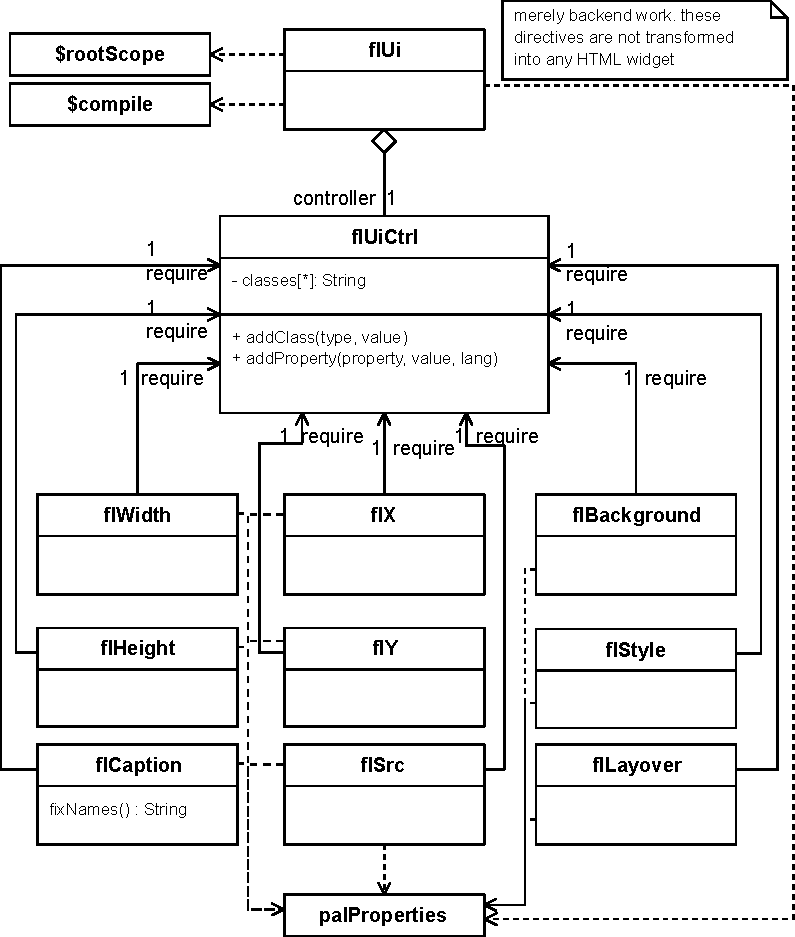
\includegraphics{figures/design-class-ui.pdf}
    \caption{Class Diagram: UI}
    \label{fig:class-ui}
\end{figure}

\begin{sidewaysfigure}[htb]
    \centering
    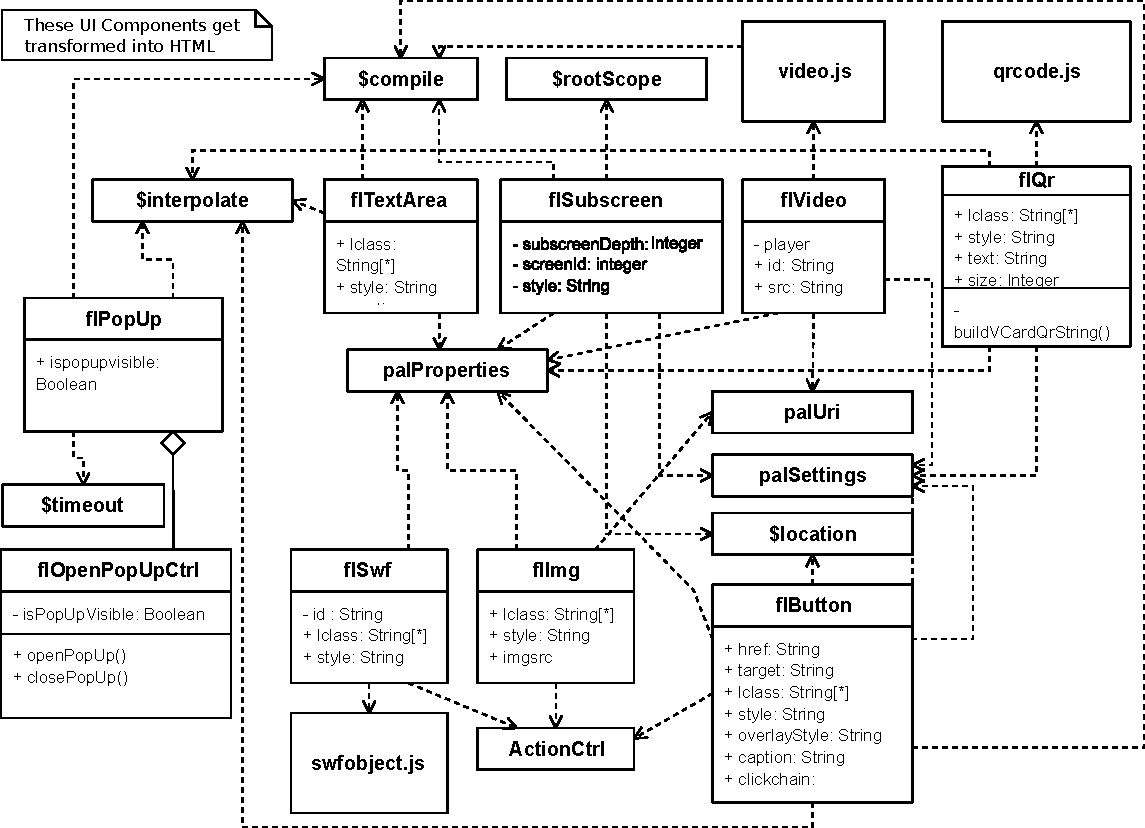
\includegraphics{figures/design-class-uicomponent.pdf}
    \caption{Class Diagram: UI Component}
    \label{fig:class-uicomponent}
\end{sidewaysfigure}

\begin{sidewaysfigure}[htb]
    \centering
    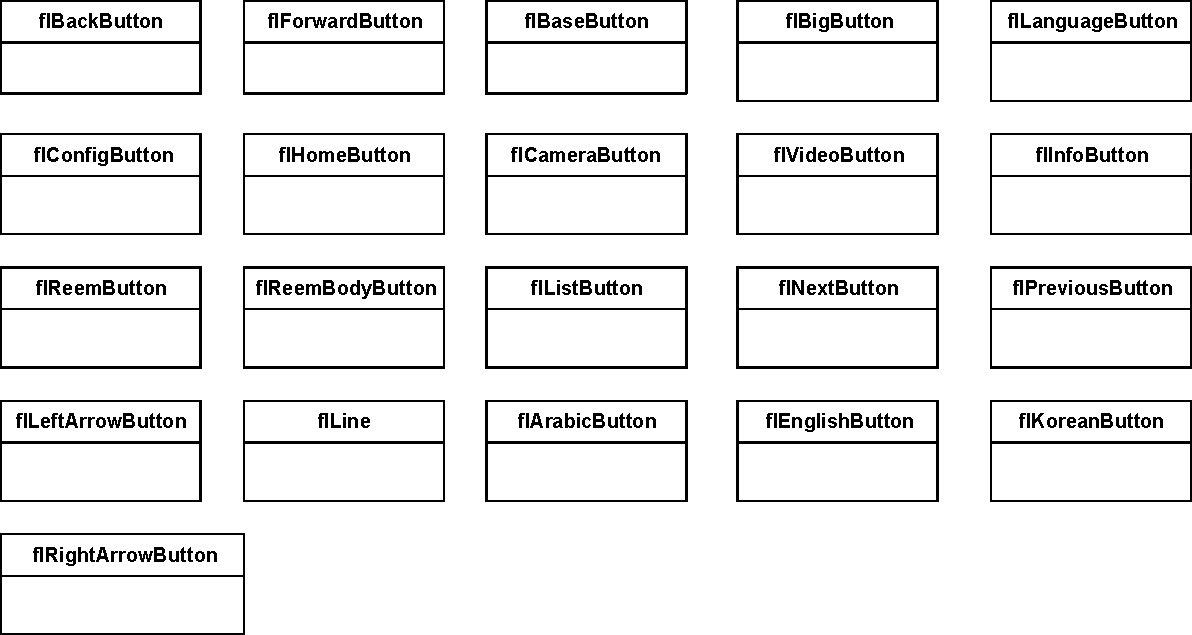
\includegraphics{figures/design-class-themecomponents.pdf}
    \caption{Class Diagram: UI Theme Component}
    \label{fig:class-themecomponent}
\end{sidewaysfigure}

\begin{figure}[htb]
    \centering
    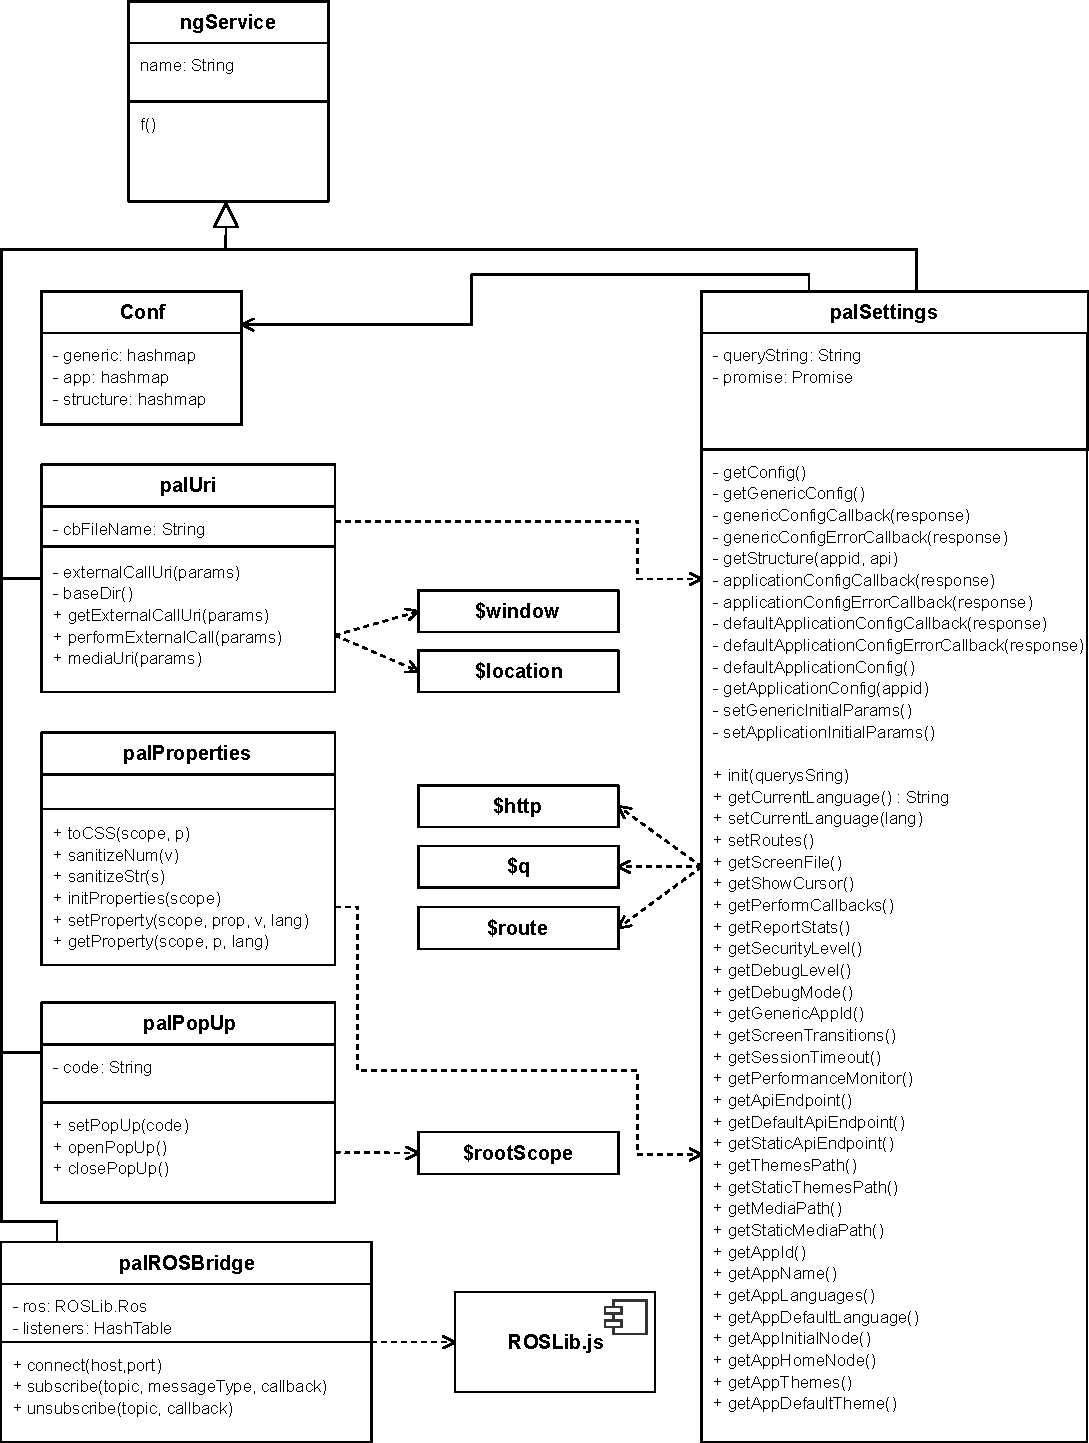
\includegraphics{figures/design-class-services.pdf}
    \caption{Class Diagram: UI services}
    \label{fig:class-services}
\end{figure}

\begin{figure}[htb]
    \centering
    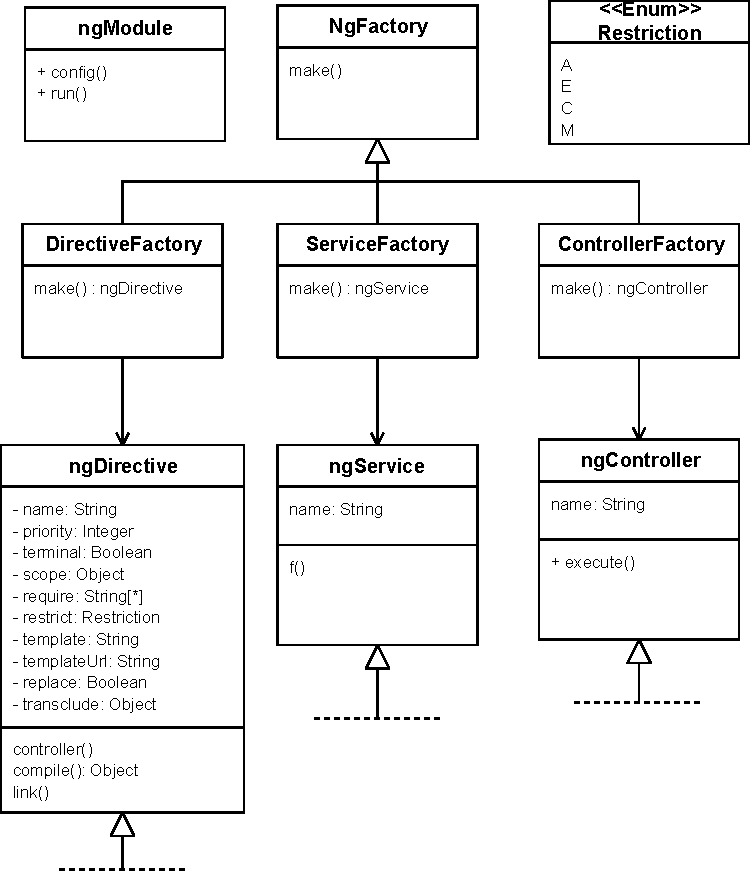
\includegraphics{figures/design-class-ngfactory.pdf}
    \caption{Class Diagram: Angular factory}
    \label{fig:class-ngfactory}
\end{figure}

\begin{figure}[htb]
    \centering
    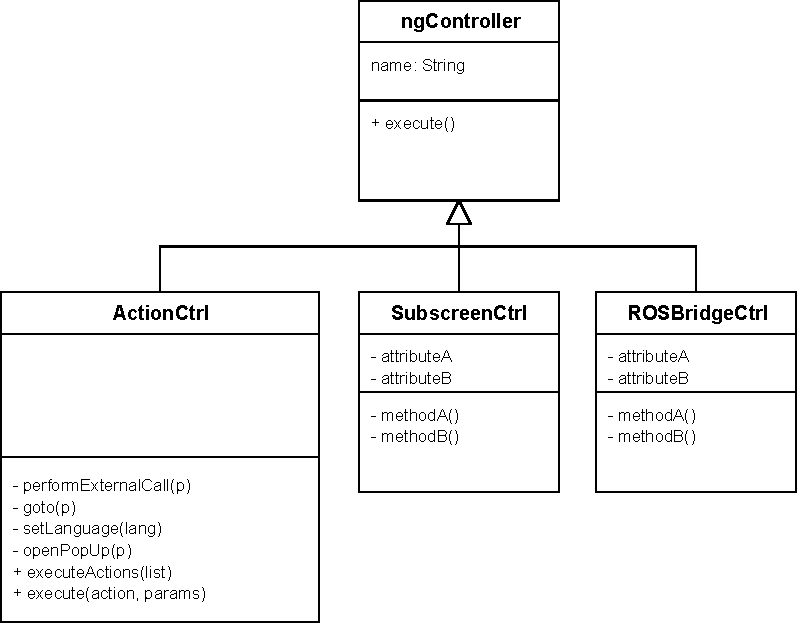
\includegraphics{figures/design-class-controllers.pdf}
    \caption{Class Diagram: Angular controllers}
    \label{fig:class-controllers}
\end{figure}

\begin{figure}[htb]
    \centering
    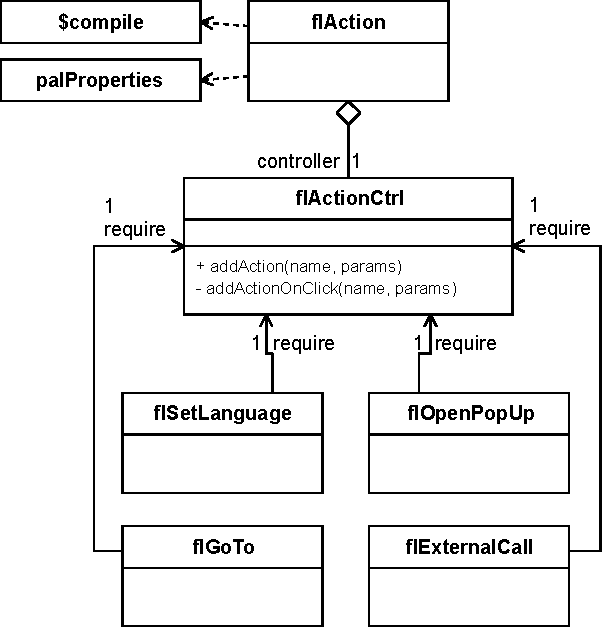
\includegraphics{figures/design-class-action.pdf}
    \caption{Class Diagram: UI action}
    \label{fig:class-action}
\end{figure}


% ********** PACKAGE DIAGRAM ********
\FloatBarrier
\subsection{Packages Diagrams}
The notion of package is implemented with Angular modules.
Modules can have an array of dependencies.

\begin{figure}[htb]
    \centering
    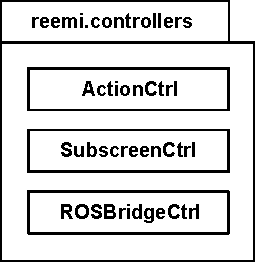
\includegraphics{figures/design-package-controllers.pdf}
    \caption{Packages Diagram: Controllers}
    \label{fig:pkg-controllers}
\end{figure}

\begin{figure}[htb]
    \centering
    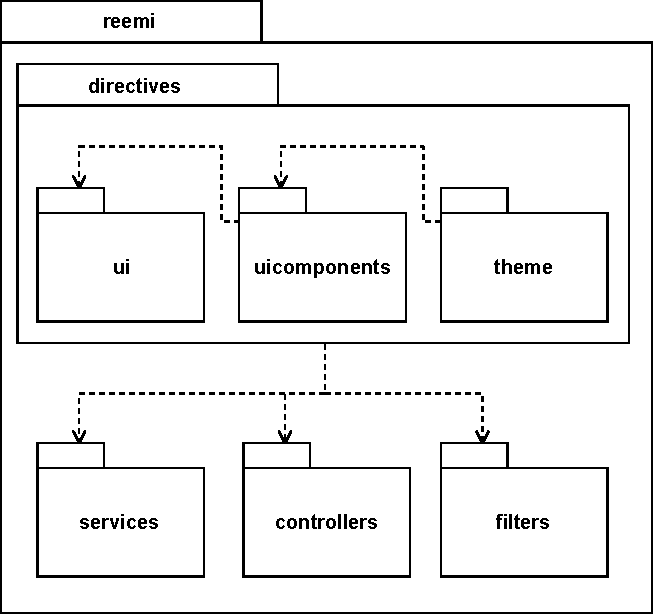
\includegraphics{figures/design-package-reemi.pdf}
    \caption{Packages Diagram: Application}
    \label{fig:pkg-reemi}
\end{figure}

\begin{figure}[htb]
    \centering
    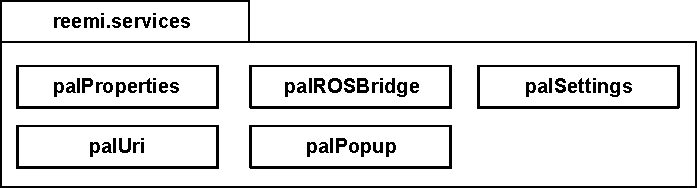
\includegraphics{figures/design-package-services.pdf}
    \caption{Packages Diagram: Services}
    \label{fig:pkg-services}
\end{figure}

\begin{figure}[htb]
    \centering
    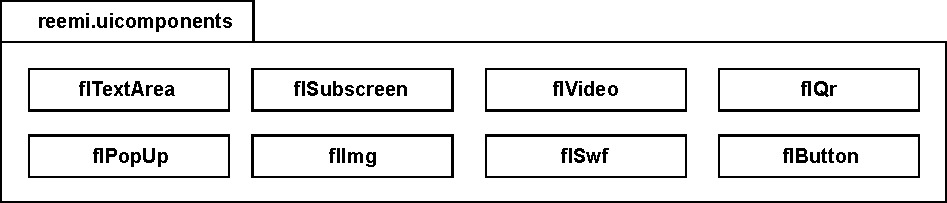
\includegraphics{figures/design-package-uicomponents.pdf}
    \caption{Packages Diagram: UI components}
    \label{fig:pkg-uicomponents}
\end{figure}

\begin{figure}[htb]
    \centering
    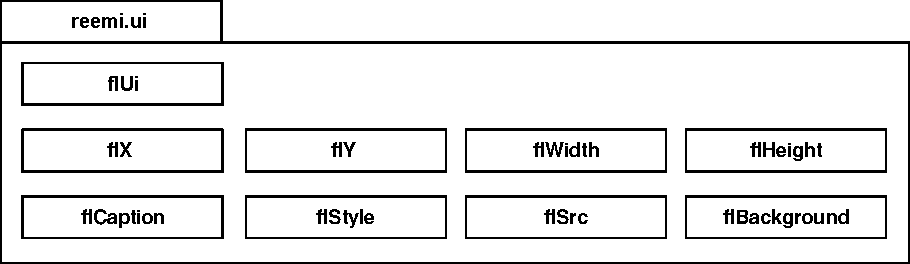
\includegraphics{figures/design-package-ui.pdf}
    \caption{Packages Diagram: UI}
    \label{fig:pkg-ui}
\end{figure}

\begin{figure}[htb]
    \centering
    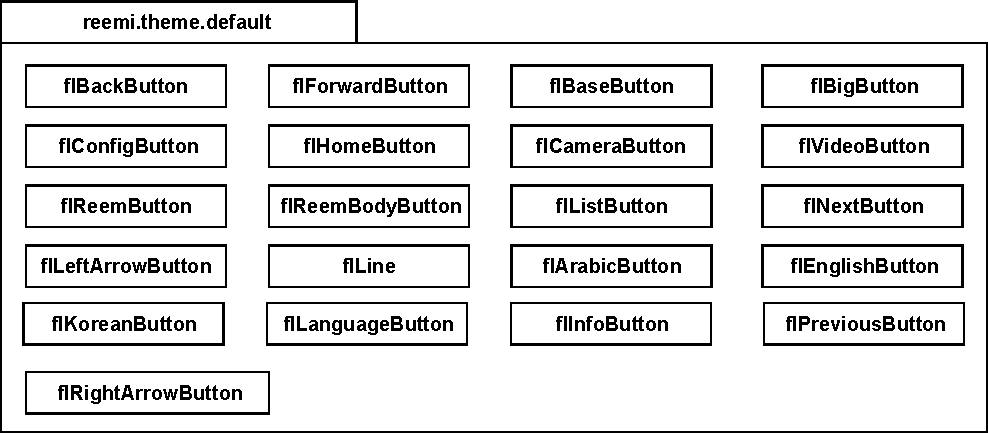
\includegraphics{figures/design-package-uithemecomponents.pdf}
    \caption{Packages Diagram: UI theme components}
    \label{fig:pkg-themecomponents}
\end{figure}

\FloatBarrier

\section{Dynamic View}
This section contains a detailed description of the most relevant operations.
They are grouped in 7 FIXME categories: boot-strap and configuration, handling properties and transformation to \ac{HTML}, pop-ups, internal navigation and communication with ROS Bridge.
It always works the same way: writing the appropriate behaviour in directives (controller, compile and link functions) and injecting the required services following the flow that Angular needs.

\subsection{Boot-strap and Configuration}
During the boot-strap process of Angular, the system performs some key operations, like registering modules, setting dependencies and the default routes \\ (e.g. \texttt{http:// ... /app/index.html\#/products-view/14/detail-view}.
The Flango \cm also fetches de configuration from the backend and builds the local object that represents it.
Figures \ref{fig:design-seqdia-bootstrap-1}, \ref{fig:design-seqdia-bootstrap-2} and \ref{fig:design-seqdia-bootstrap-3}, show the bootstrap of the program.

\begin{figure}[htb]
    \centering
    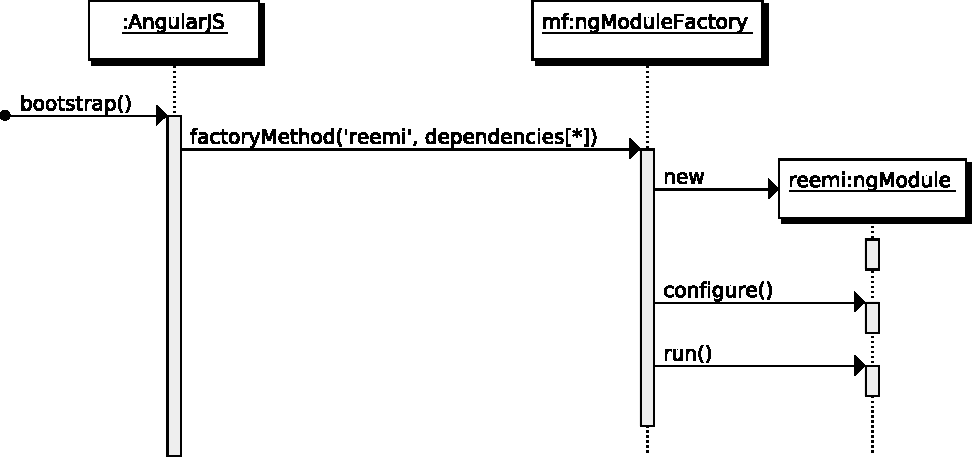
\includegraphics{figures/design/seqdia/bootstrap-1.pdf}
    \caption{Sequence Diagram: Bootstrap 1}
    \label{fig:design-seqdia-bootstrap-1}
\end{figure}

\begin{figure}[htb]
    \centering
    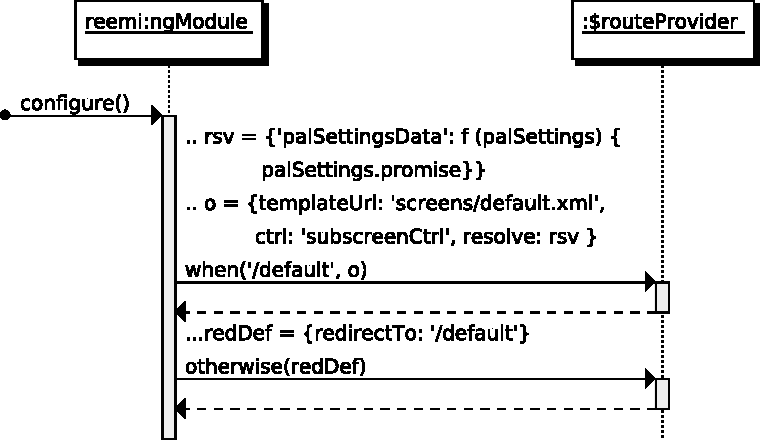
\includegraphics{figures/design/seqdia/bootstrap-2.pdf}
    \caption{Sequence Diagram: Bootstrap 2}
    \label{fig:design-seqdia-bootstrap-2}
\end{figure}

\begin{figure}[htb]
    \centering
    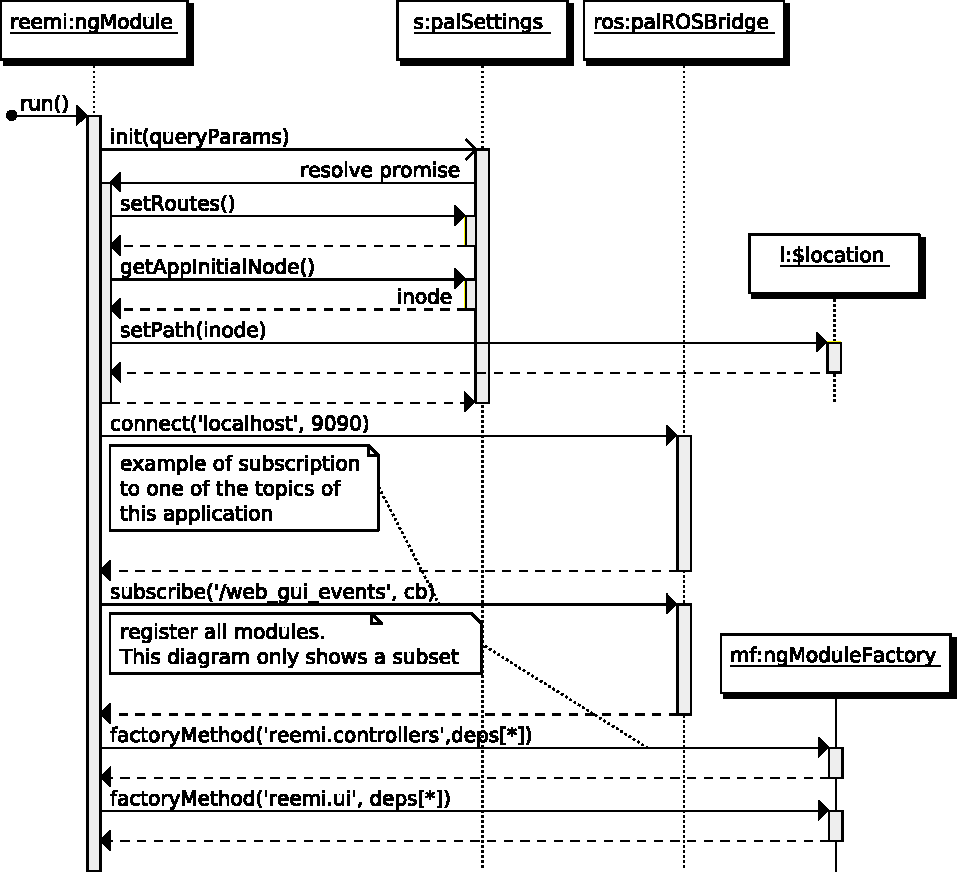
\includegraphics{figures/design/seqdia/bootstrap-3.pdf}
    \caption{Sequence Diagram: Bootstrap 3}
    \label{fig:design-seqdia-bootstrap-3}
\end{figure}

The configuration is encapsulated in the \texttt{palSettings} angular service which, like all services in Angular, is a singleton.
It is created with a factory: when a new instance of \texttt{palSettings} is to be created, it runs some code that prepares an object to return, the instance itself.
The bootstrap process, there is a call \lstinline$palSettings.init(queryString)$ (\fref{fig:design-seqdia-palSettings-init}).
This method fetches the configuration from the backend using an asynchronous call (\fref{fig:design-seqdia-palSettings-getConfig}) which, in turn, delegates to other internal operations.
To avoid errors, the system uses \emph{deferred promises}: the \texttt{init} method returns an object immediately and it receives a notification when all asynchronous calls have been completed, that is, when the configuration object is ready to be used in the application.

The configuration object has three parts: the generic configuration (paths, \ac{API} endpoint, etc) \fref{fig:design-seqdia-palSettings-getGenericConfig}, the application specific configuration {fig:design-seqdia-palSettings-getApplicationConfig} (available languages, available themes, default language, etc) and the structure \fref{fig:design-seqdia-palSettings-getStructure} (a graph that matches screens with \ac{URI}.
It degrades gradually: it first tries to fetch the real application, if it fails attempts to fetch the default application \fref{fig:design-seqdia-palSettings-defaultApplicationConfig}, if this is not possible, it obtains the static application shipped with the program (See \texttt{errorCallback} in \fref{fig:design-seqdia-palSettings-defaultApplicationConfig}).

\paragraph{Promises and deferred objects} Futures, promises and delays are constructs for synchronising in a programming language.
\textit{Promises} were introduced by Daniel P. Friedman and David Wise in 1977, \textit{futures} in 1977 by Henry Baker and Carl Hewitt.
The term promise was coined by Liskov and Shrira \cite{Liskov:1988} in 1988.

The three words are often used interchangeably although they have some differences:
\begin{itemize}
\item Future: read-only placeholder view of a variable
\item Promise: writeable, single assignment container that sets the value of the future.
\end{itemize}
Essentially, promises represent the result of a task that might have not been completed, something very common in JavaScript.
Asynchronous calls are normally handled with callbacks (see \fref{chap:implementation}).
However, when there are nested or concurrent asynchronous calls, like the case of fetching the configuration from the \flangobe , callbacks become hard to maintain.
A solution is defining a promise at the beginning and \emph{resolving} it when all calls are completed (or \emph{rejecting} it when a sufficient number of calls have failed).
This way functions can be decoupled and testing is easier. 

\begin{figure}[htb]
    \centering
    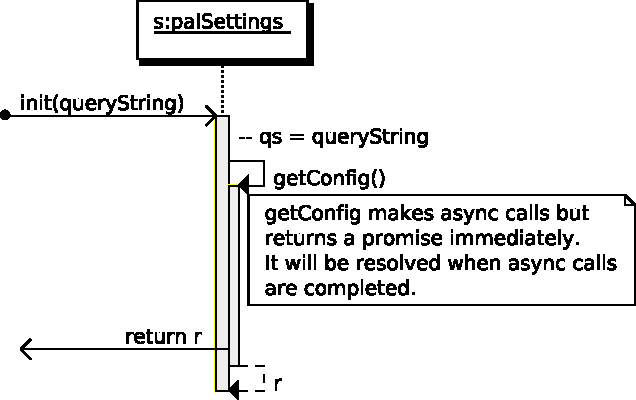
\includegraphics{figures/design/seqdia/palSettings-init.pdf}
    \caption{Sequence Diagram: init()}
    \label{fig:design-seqdia-palSettings-init}
\end{figure}

\begin{figure}[htb]
    \centering
    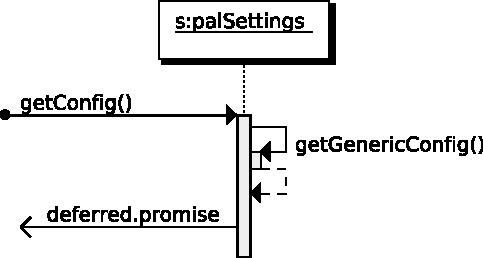
\includegraphics{figures/design/seqdia/palSettings-getConfig.pdf}
    \caption{Sequence Diagram: getConfig()}
    \label{fig:design-seqdia-palSettings-getConfig}
\end{figure}

\begin{figure}[htb]
    \centering
    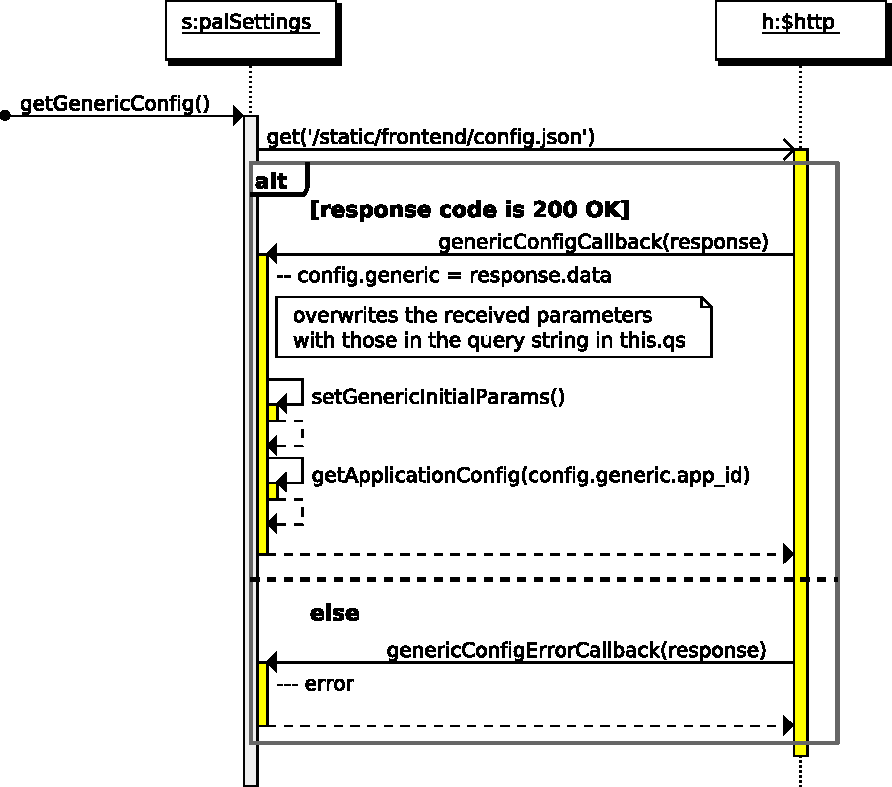
\includegraphics{figures/design/seqdia/palSettings-getGenericConfig.pdf}
    \caption{Sequence Diagram: getGenericConfig()}
    \label{fig:design-seqdia-palSettings-getGenericConfig}
\end{figure}

\begin{figure}[htb]
    \centering
    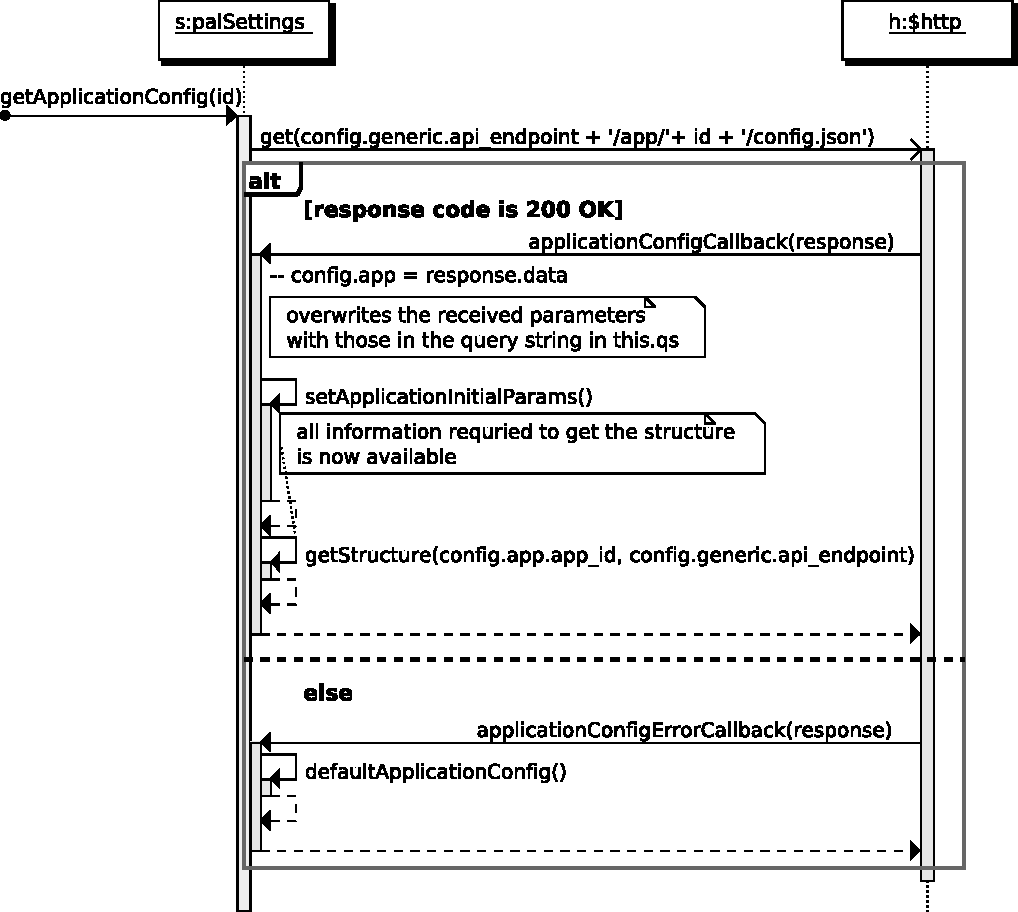
\includegraphics{figures/design/seqdia/palSettings-getApplicationConfig.pdf}
    \caption{Sequence Diagram: getApplicationConfig()}
    \label{fig:design-seqdia-palSettings-getApplicationConfig}
\end{figure}


\begin{figure}[htb]
    \centering
    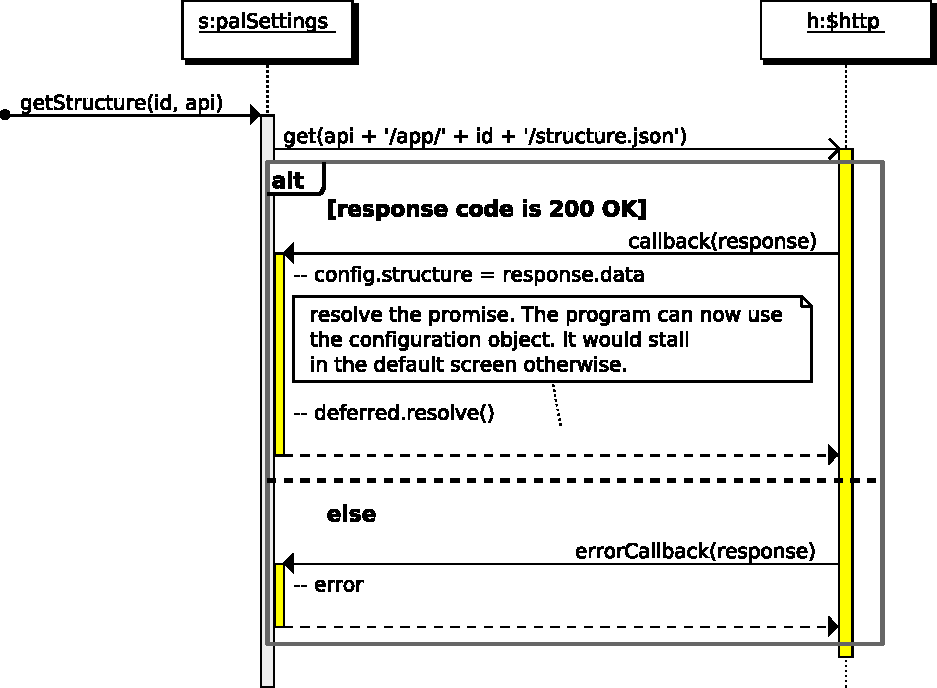
\includegraphics{figures/design/seqdia/palSettings-getStructure.pdf}
    \caption{Sequence Diagram: getStructure()}
    \label{fig:design-seqdia-palSettings-getStructure}
\end{figure}

\begin{figure}[htb]
    \centering
    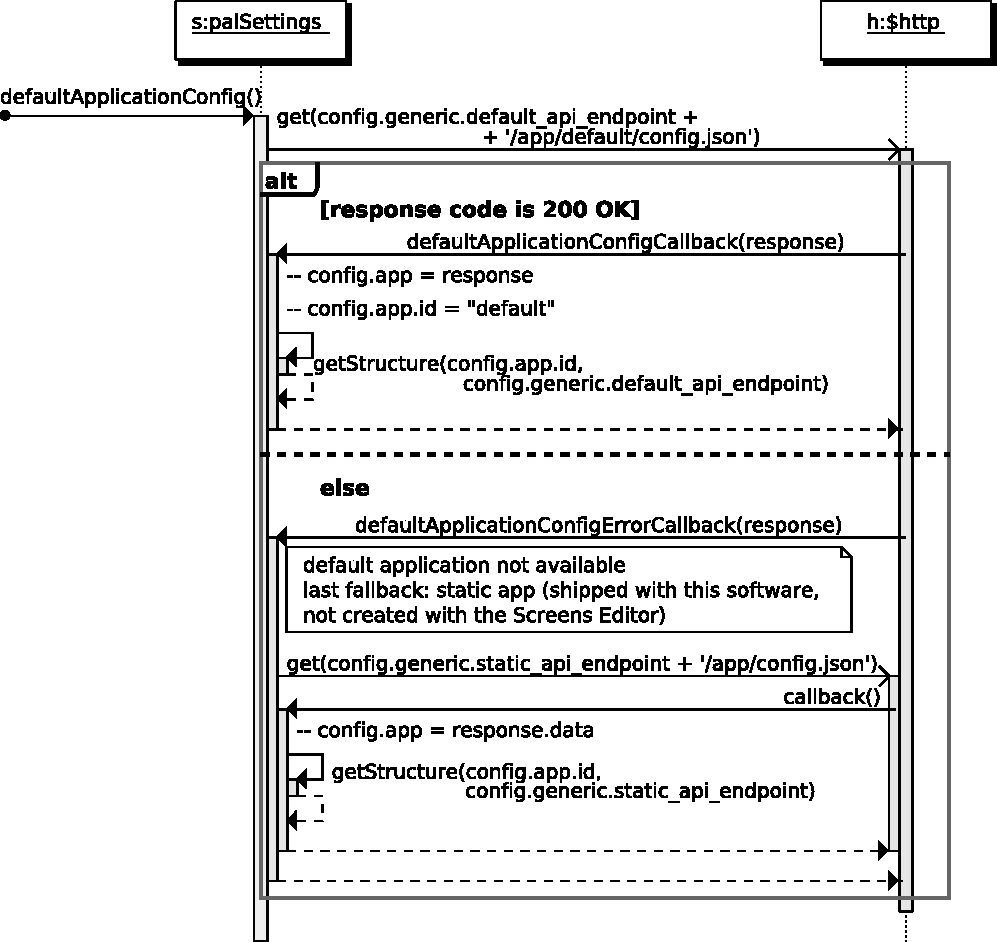
\includegraphics{figures/design/seqdia/palSettings-defaultApplicationConfig.pdf}
    \caption{Sequence Diagram: defaultApplicationConfig()}
    \label{fig:design-seqdia-palSettings-defaultApplicationConfig}
\end{figure}

\FloatBarrier

\subsection{Properties management and transformation to \acs{HTML}}
Browsers can only parse \ac{HTML} nodes.
When the parser finds an \ac{XML} node, it prints the inner text node because \ac{HTML} also has text nodes.
With Angular \ac{XML} nodes can have behaviour: it teaches the browser new syntax.
For example, \\ \lstinline$<fl:ui fl:base-button fl:x="100" fl:width="90"></ui>$ triggers the directive \\ \lstinline$flBaseButton$, which encapsulates the behaviour to transform it to \ac{HTML}: \\ \lstinline$<a href="..."><div>text</div></a>$.

To expose values to the view, Angular attaches an object \texttt{\$scope} to all directives  \fref{fig:design-properties-management}.
A scope can be \textbf{isolated}, \textbf{prototypically inherited} from the parent, or \textbf{shared} with other directives of the same type.
This project uses the scope to encapsulate the properties extracted or inferred from the \ac{XML} node.
Thus, any element \lstinline$<fl:ui>$ or concrete types \lstinline$base-button$, \lstinline$back-button$, etc has a \texttt{scope} object attached that contains all the necessary data to render an \ac{HTML} node.
Scopes are also watched to provide two-way data binding with controllers (see \fref{fig:mvc-with-observer})

\begin{figure}[h]
    \centering
    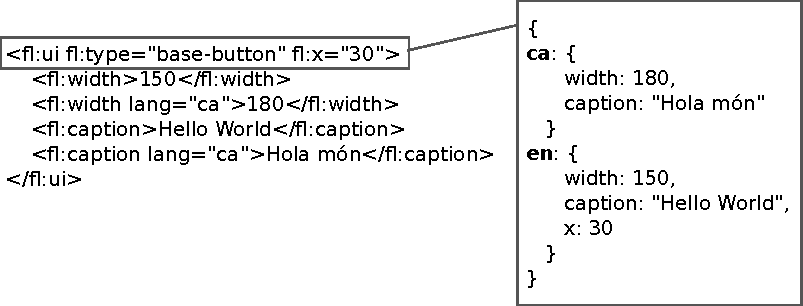
\includegraphics{figures/design/properties-management.pdf}
    \caption{Scope object attached to a node}
    \label{fig:design-properties-management}
\end{figure}

\lstinputlisting[language=xml, caption={Original XML BaseButton}, label=design-real-xml-button]{src/from-xml-to-html-1.xml}
\lstinputlisting[language=JavaScript, caption={Properties object}, label=design-scope-properties]{src/from-xml-to-html-properties.js}

\begin{figure}
    \centering
    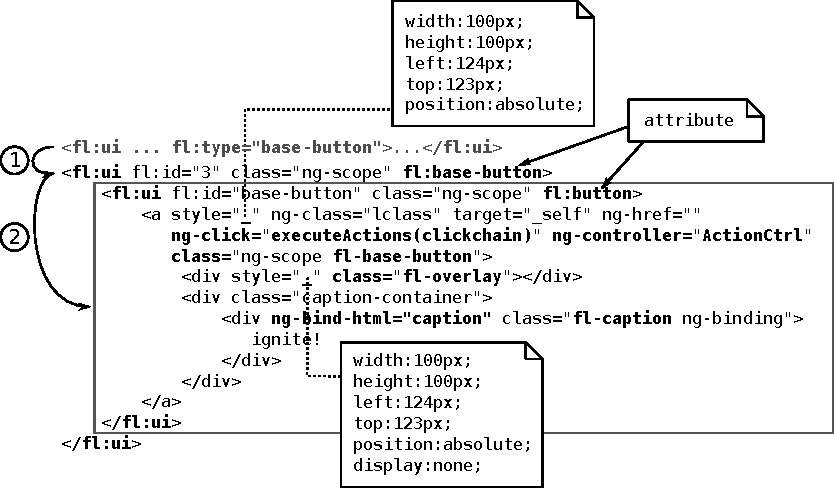
\includegraphics{figures/design/from-xml-to-html-3.pdf}
    \caption{Transformation from \acs{XML} to \acs{HTML} and styles management}
    \label{fig:design-xml-to-html-3}
\end{figure}

Directives can be \textbf{restricted} to \textbf{Element}, \textbf{Attribute}, \textbf{Class} or \textbf{coMment} \fref{fig:class-ngfactory}.
Flango \cm is designed to adapt to this syntax and to decouple and reuse elements as much as possible.
All UI Components have the tag \lstinline$<fl:ui>$ and an attribute \lstinline$fl:type$ that defines the concrete type.
Instead of having all behaviour in one directive \texttt{fl:ui} (restricted to Element), it uses \texttt{flUi} to rewrite the \ac{DOM}:\\
\lstinline$<fl:ui fl:type="base-button"></ui>$ becomes \\ \lstinline$<fl:ui base-button></ui>$, where \texttt{base-button} is an attribute of the element \texttt{fl:ui}.
There is a directive \texttt{flBaseButton} (restricted to Attribute) that encapsulates the behaviour of this tag.
Likewise, it initialises the properties object for this \texttt{ui} element and stores the type that will be later used as a value for the \texttt{class} attribute in the \ac{HTML} element.
The stylesheet of the theme defines the inheritance of styles: a base-button is implemented with a button and, therefore, inherits all properties of the class \texttt{button}.

\Fref{fig:design-xml-to-html-3} shows the transformation of a base button in the \ac{XML} screen (listing \ref{design-real-xml-button}) and the use of the properties object in the scope (listing \ref{design-scope-properties}).

The algorithm to decide the properties for an object and draw it with \ac{HTML} goes with the flow of the framework:
\begin{enumerate}
	\item With directive \texttt{flUi}: Create an attribute with the value of the \texttt{type} attribute \fref{fig:design-seqdia-ui-compile}. Initialise the properties object in the controller \fref{fig:design-seqdia-ui-controller} The framework compiles and links the rest of the code (e.g. the \texttt{link()} function in inner \texttt{width} tags to read values of inner tags (\fref{fig:design-seqdia-width-link}))
	\item With directive \texttt{flUi} link function (\fref{fig:design-seqdia-ui-link}), read in-line attributes. Because it reads everything recursively, this is the last function to run. Properties are only set if they have not been set yet: inner tags (more specific) have higher priority than in-line attributes. Recompile the directive to make angular find it. 
	\item With the new directive (e.g. \texttt{flBaseButton}), run component-specific behaviour. \texttt{flUi} does not have a \texttt{type} attribute anymore and is ignored. Specific behaviour can be transforming it using a template (\fref{fig:design-seqdia-basebutton-link}). Recompile (e.g. the template might, and normally has, tags that can trigger angular directives).
	\item Eventually reach a base component and run component-specific behaviour, e.g. create \ac{HTML} nodes that can actually draw the UI Component.
\end{enumerate}

\begin{figure}[htb]
    \centering
    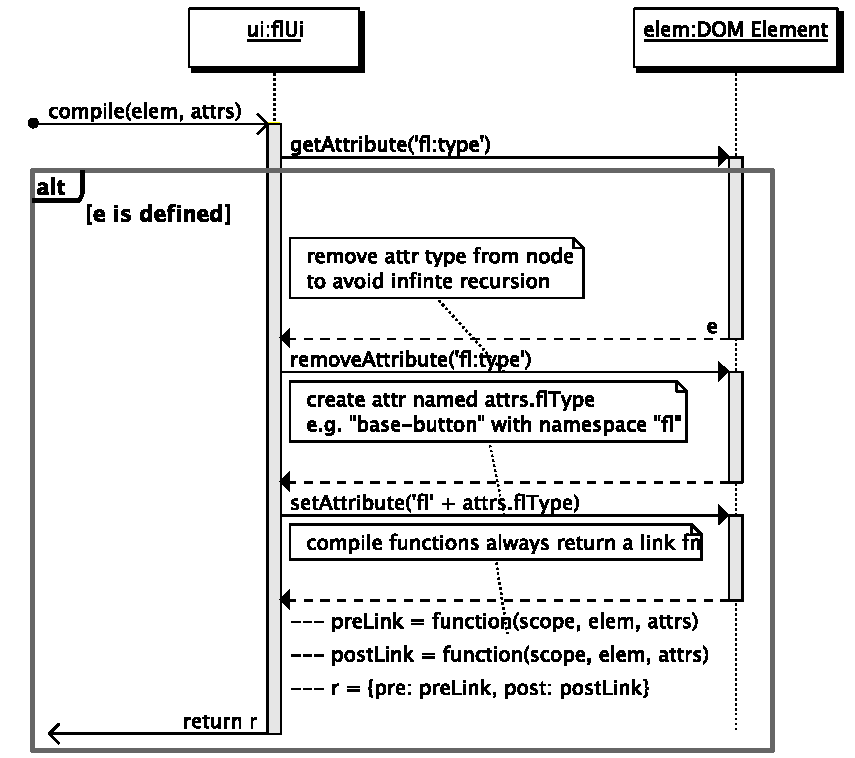
\includegraphics{figures/design/seqdia/ui-compile.pdf}
    \caption{Sequence Diagram: flUi::compile}
    \label{fig:design-seqdia-ui-compile}
\end{figure}

\begin{figure}[htb]
    \centering
    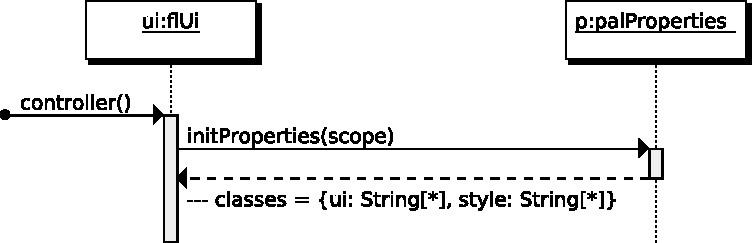
\includegraphics{figures/design/seqdia/ui-controller.pdf}
    \caption{Sequence Diagram: flUi::controller}
    \label{fig:design-seqdia-ui-controller}
\end{figure}

\begin{figure}[htb]
    \centering
    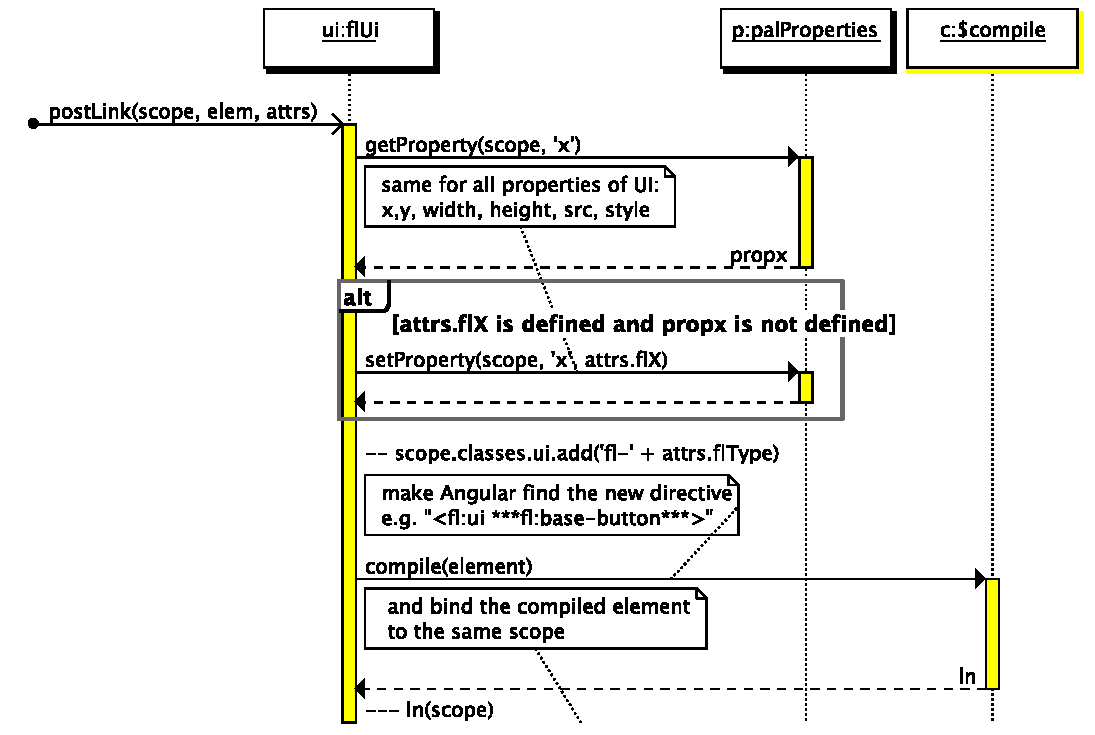
\includegraphics{figures/design/seqdia/ui-link.pdf}
    \caption{Sequence Diagram: flUi::link}
    \label{fig:design-seqdia-ui-link}
\end{figure}

\begin{sidewaysfigure}[htb]
    \centering
    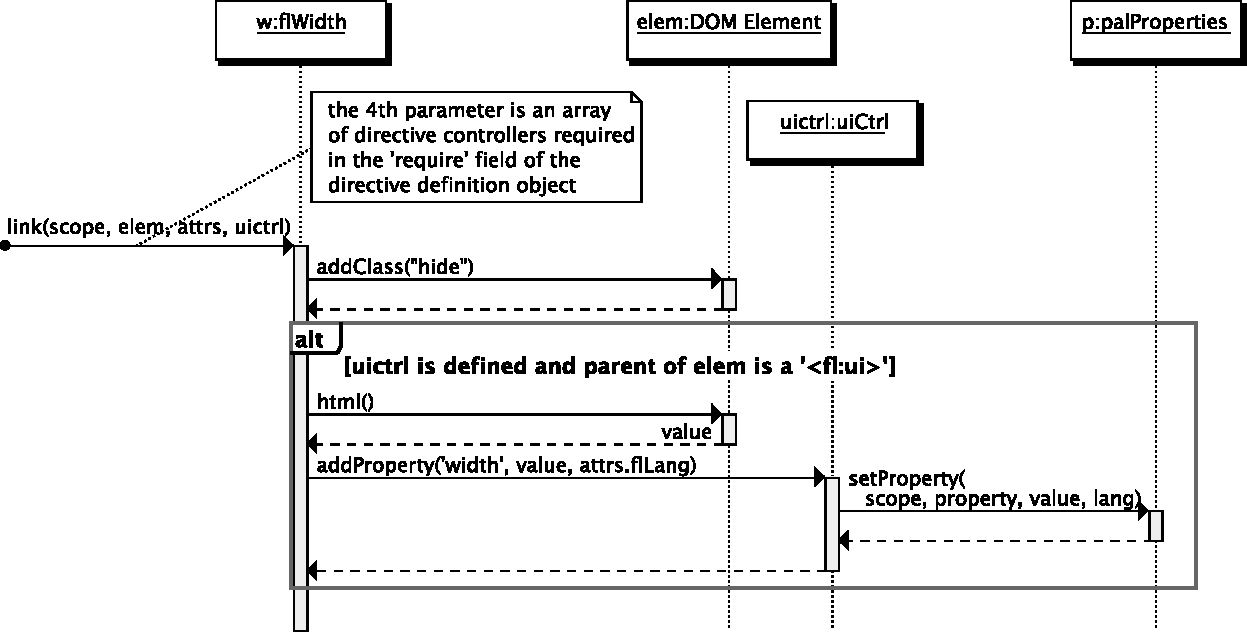
\includegraphics{figures/design/seqdia/width-link.pdf}
    \caption{Sequence Diagram: flWidth::link}
    \label{fig:design-seqdia-width-link}
\end{sidewaysfigure}

\begin{figure}[htb]
    \centering
    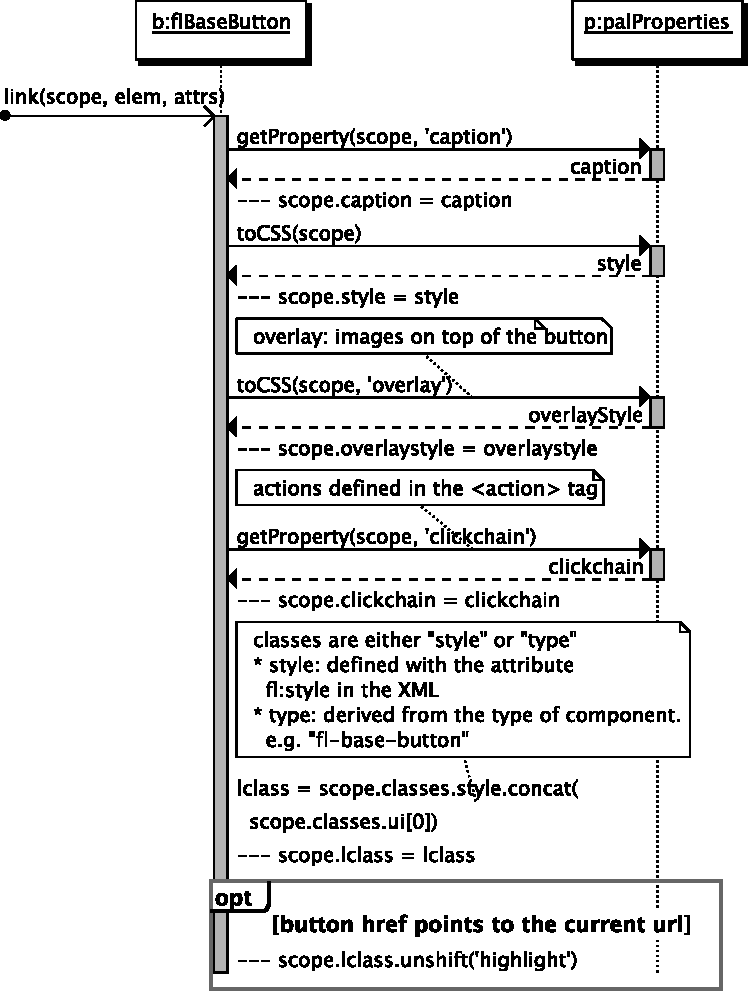
\includegraphics{figures/design/seqdia/basebutton-link.pdf}
    \caption{Sequence Diagram: flBaseButton::link}
    \label{fig:design-seqdia-basebutton-link}
\end{figure}

\lstinline$<fl:ui base-button>...</ui>$ eventually becomes \\
\lstinline$<div class="base-button" style="...">...</div>$. 
With this rewrite strategy the directive eventually outputs real \ac{HTML} that defines the structure of the UI Component and uses the style sheet.

All UI Components have an  \textbf{\ac{HTML} template} that defines their structure, a \textbf{\ac{CSS} class} that defines their style, \textbf{in-line \ac{CSS}} that defines their exclusive properties (e.g. position, size...) and they are binded to \textbf{\texttt{ActionCtrl}} to expose behaviour (e.g. on click).
\FloatBarrier

\paragraph{Inheritance and composition} UI Components can be composited: a \texttt{home-button} is implemented with a \texttt{base-button}, which in turn it is implemented with a \texttt{button}, that eventually becomes \ac{HTML}.
Each component can have defaults for properties.
For instance, if \texttt{base-button} has a \texttt{width} of 100px in the template, and a component that is implemented with \texttt{base-button} (e.g. \texttt{home-button}) does not define a different with, it sets \texttt{width} to 100 in the properties object.
This behaviour is achieved with the \texttt{compile} and \texttt{link} functions of directives.
Language-specific properties are decided the same way: it attempts to use current language properties, if they are not defined, it falls back to the default language.

\subsection{Actions execution}
Buttons and other UI Components, like images or QR Codes, respond to clicks.
\ac{XML} can define a list of actions to execute (e.g. set the language, open a popup, go to \ac{URI}...)
The controller ActionCtrl encapsulates the logic to process these commands.

\lstinputlisting[language=xml, caption={A list of actions in \ac{XML}}]{src/example-actions.xml}

\lstinputlisting[language=xml, caption={Result button (snippet)}]{src/example-result-button-action.html}

To create the list of actions, when the component is clicked it runs \lstinline$executeActions()$, which has a list of actions to execute as a parameter using the \emph{command pattern}.

\begin{figure}[htb]
    \centering
    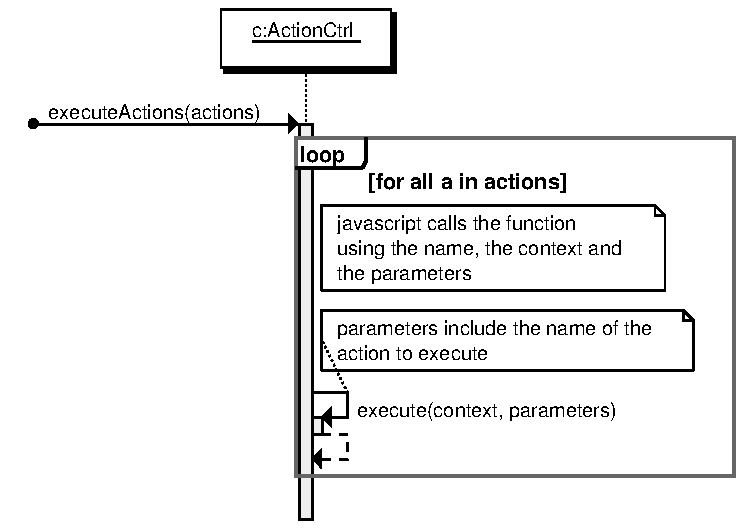
\includegraphics{figures/design/seqdia/actionCtrl-executeActions.pdf}
    \caption{Sequence Diagram: ActionCtrl::executeActions}
    \label{fig:design-seqdia-actionCtrl-executeActions}
\end{figure}

\begin{figure}[htb]
    \centering
    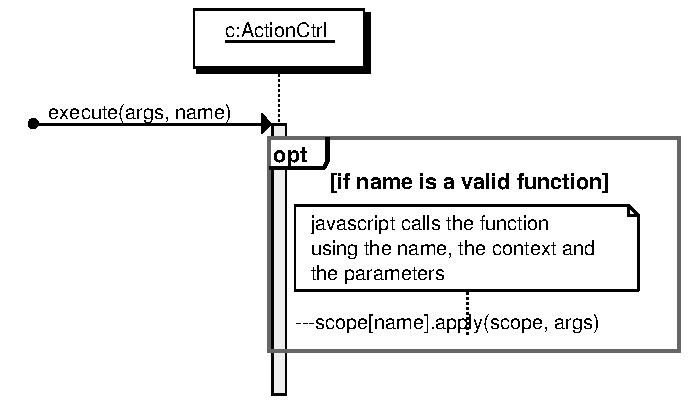
\includegraphics{figures/design/seqdia/actionCtrl-execute.pdf}
    \caption{Sequence Diagram: ActionCtrl::execute}
    \label{fig:design-seqdia-actionCtrl-execute}
\end{figure}

\begin{figure}[htb]
    \centering
    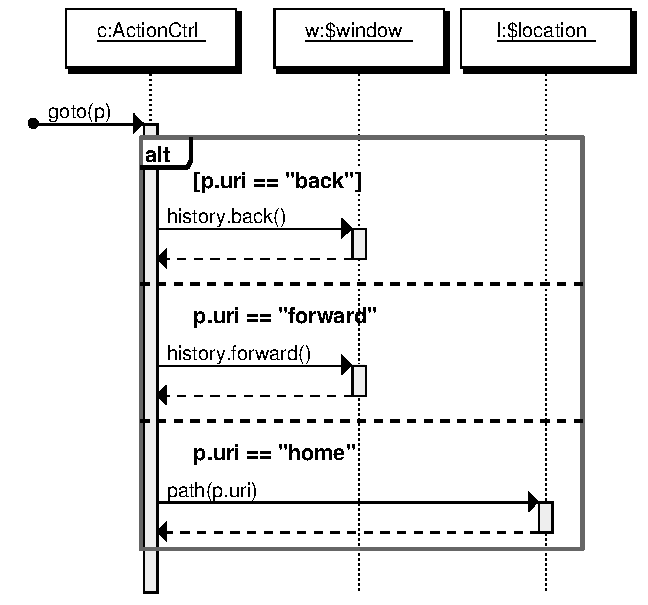
\includegraphics{figures/design/seqdia/actionCtrl-goto.pdf}
    \caption{Sequence Diagram: ActionCtrl::execute}
    \label{fig:design-seqdia-actionCtrl-goto}
\end{figure}

\FloatBarrier

%\subsection{Pop-Ups}
%description and use example

\subsection{Internal Navigation}
Angular has a navigation system based on the \acp{URL}.
The \$route service has a map that relates \acp{URL} with screens, \ac{HTML} files with directives.
On each location change, Angular looks up the destination \ac{URL} in the map to fetch the correct file.

Flango \cm composites screens with subscreens and decides the contents to show using the \ac{URL} (\fref{fig:design-internal-navigation}).
e.g. the \ac{URL} \texttt{/main-view/animals-list} does not populate the subscreen \texttt{red-panda-details}

\begin{figure}[htb]
    \centering
    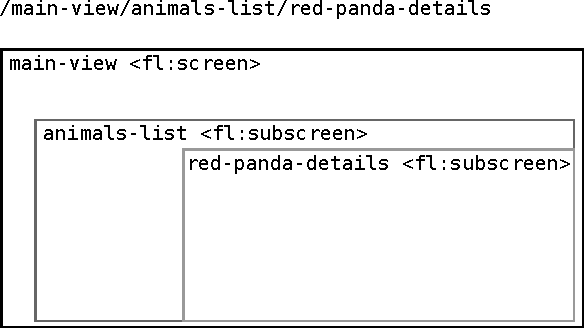
\includegraphics{figures/design/internal-navigation.pdf}
    \caption{Internal navigation with Screens and subscreens}
    \label{fig:design-internal-navigation}
\end{figure}

The behaviour of subscreens is defined in the \texttt{subscreen} directive (\fref{fig:design-seqdia-subscreen-compile}).

Only after properties of the UI Component Subscreen have been set (and the corresponding \ac{HTML} element created), Angular includes the file of the subscreen.

\begin{sidewaysfigure}[htb]
    \centering
    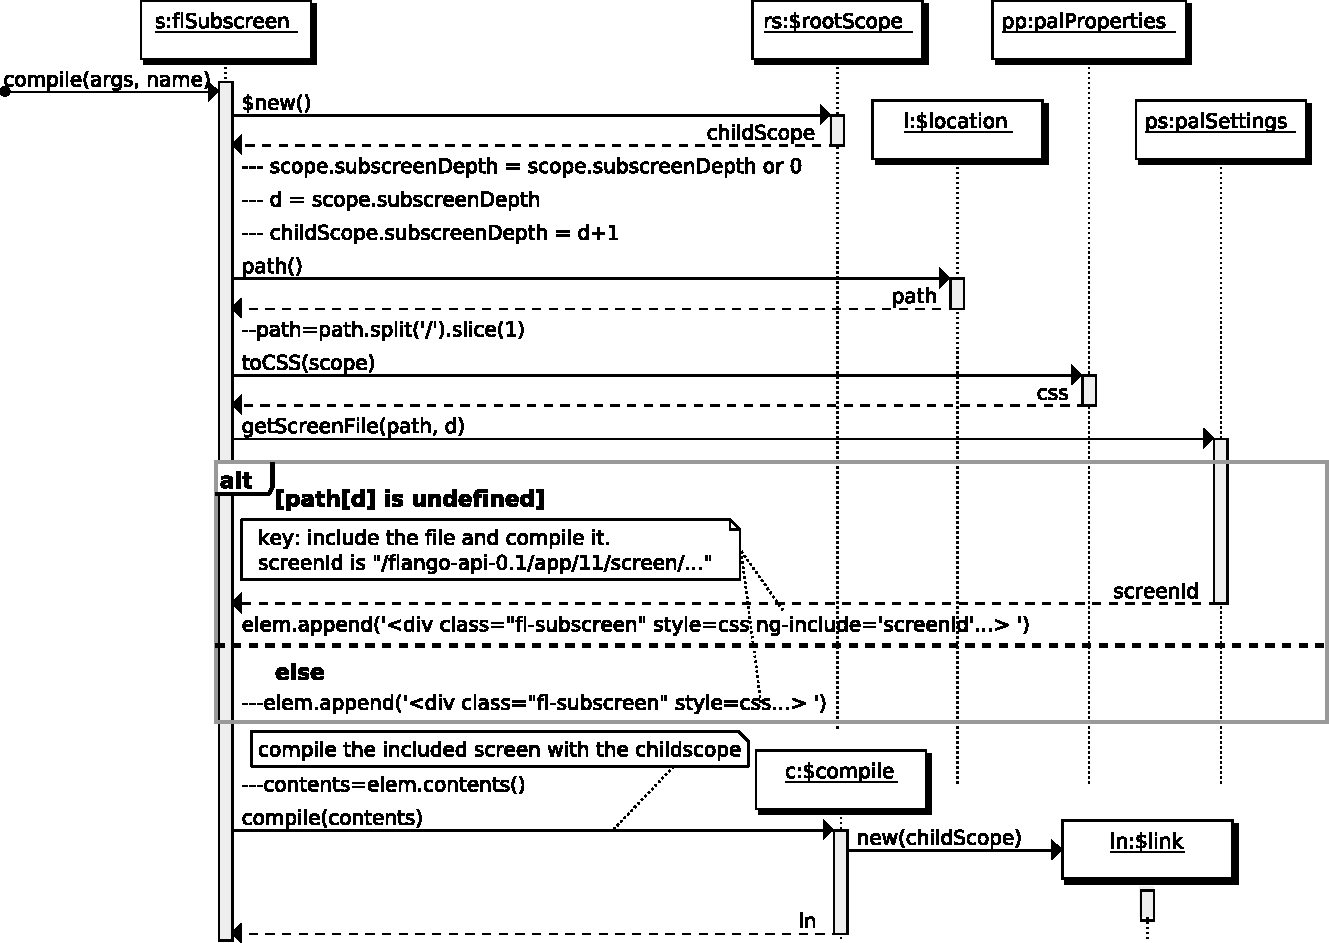
\includegraphics{figures/design/seqdia/subscreen-compile.pdf}
    \caption{Sequence Diagram: Subscreen::compile}
    \label{fig:design-seqdia-subscreen-compile}
\end{sidewaysfigure}

\begin{figure}[htb]
    \centering
    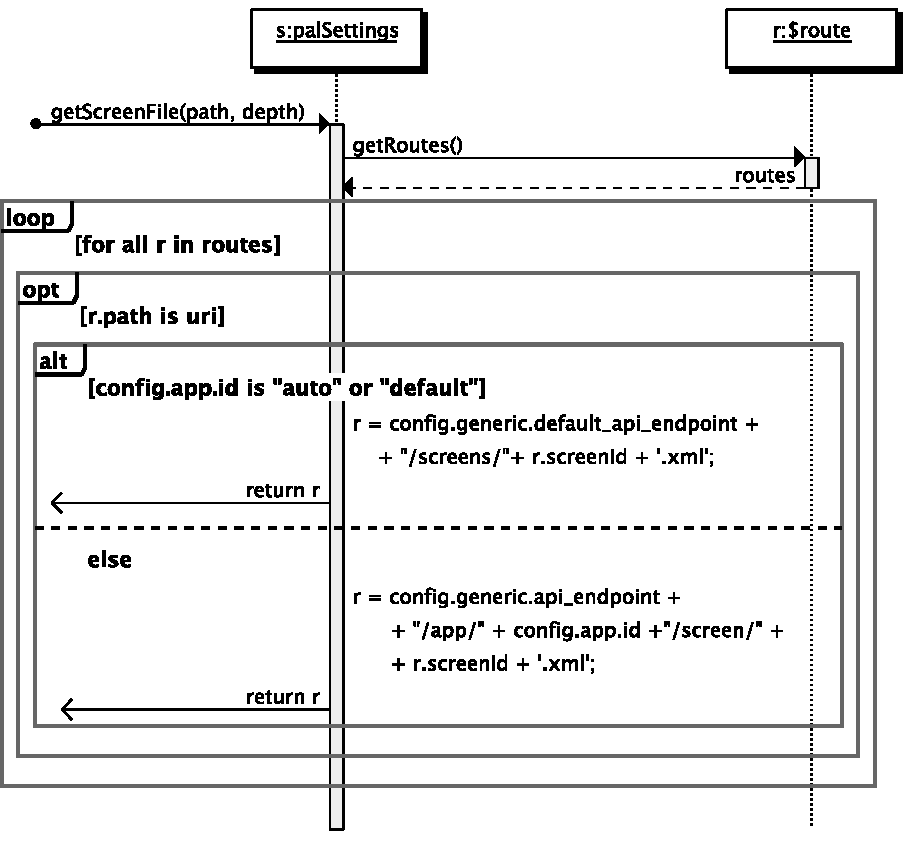
\includegraphics{figures/design/seqdia/palSettings-getScreenFile.pdf}
    \caption{Sequence Diagram: palSettings::getScreenFile}
    \label{fig:design-seqdia-palsettings-getscreenfile}
\end{figure}

\FloatBarrier

\subsection{External Calls}
FIXME motivation, rosbridge
complementa la subseccio de sota

\subsection{Responding to requests from the robot}
FIXME service, topic, rosbridge, etc.
complementa la subsecio external calls (una d'anada, una de tornada)

\begin{figure}[htb]
    \centering
    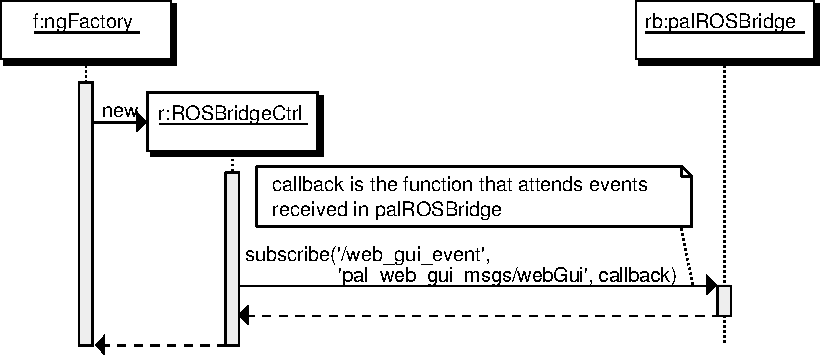
\includegraphics{figures/design/seqdia/ROSBridgeCtrl-creation.pdf}
    \caption{Sequence Diagram: ROSBridgeCtrl::instantiation and subscription to topic}
    \label{fig:design-seqdia-ROSBridgeCtrl-creation}
\end{figure}

\begin{sidewaysfigure}[htb]
    \centering
    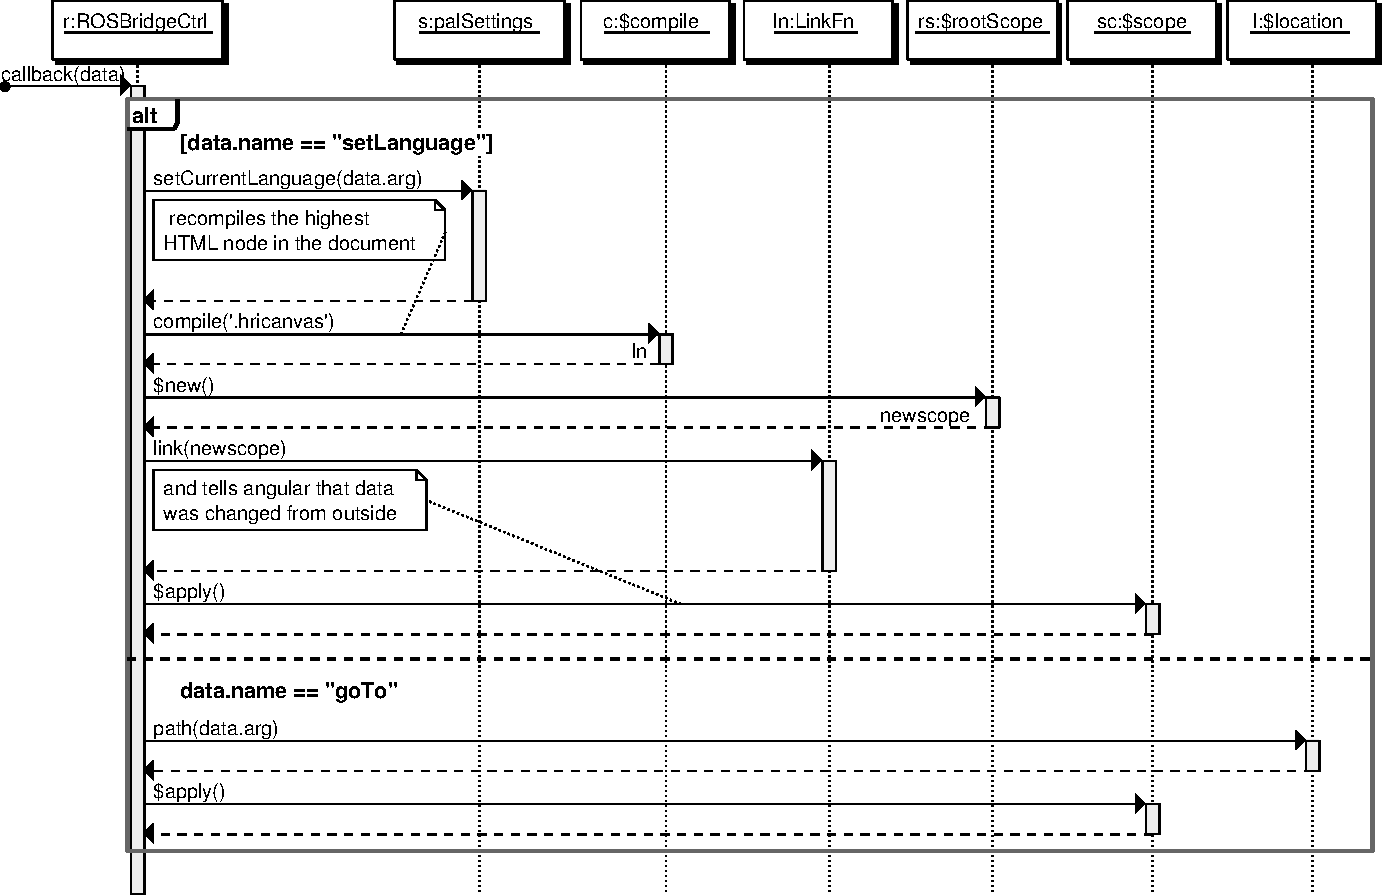
\includegraphics{figures/design/seqdia/ROSBridgeCtrl-callback.pdf}
    \caption{Sequence Diagram: ROSBridgeCtrl::Example callback function}
    \label{fig:design-seqdia-ROSBridgeCtrl-callback}
\end{sidewaysfigure}

\FloatBarrier

\section{Physical View}
This section presents a series of diagrams to illustrate the physical layout of the project: the nodes involved, the components in each node, and a clear separation of the Flango \cm and the environment.
The application is assembled in a Debian package and deployed to Basestation and the robot.
The control scripts of this package perform tasks like copying the files to the correct place (e.g. the public html folder of the web server), initialise data in the backend, etc.
The diagrams in this section show the system after the installation.

% ****** deployment *******
\begin{figure}[htb]
    \centering
    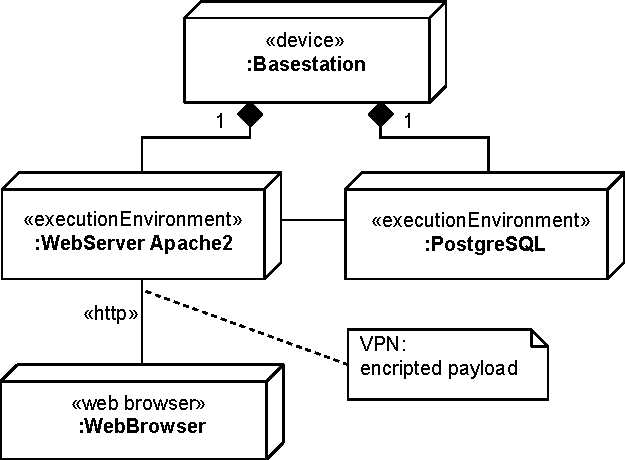
\includegraphics{figures/design-deployment-basestation.pdf}
    \caption{Deployment Diagram: Basestation}
    \label{fig:deploy-basestation}
\end{figure}

\begin{figure}[htb]
    \centering
    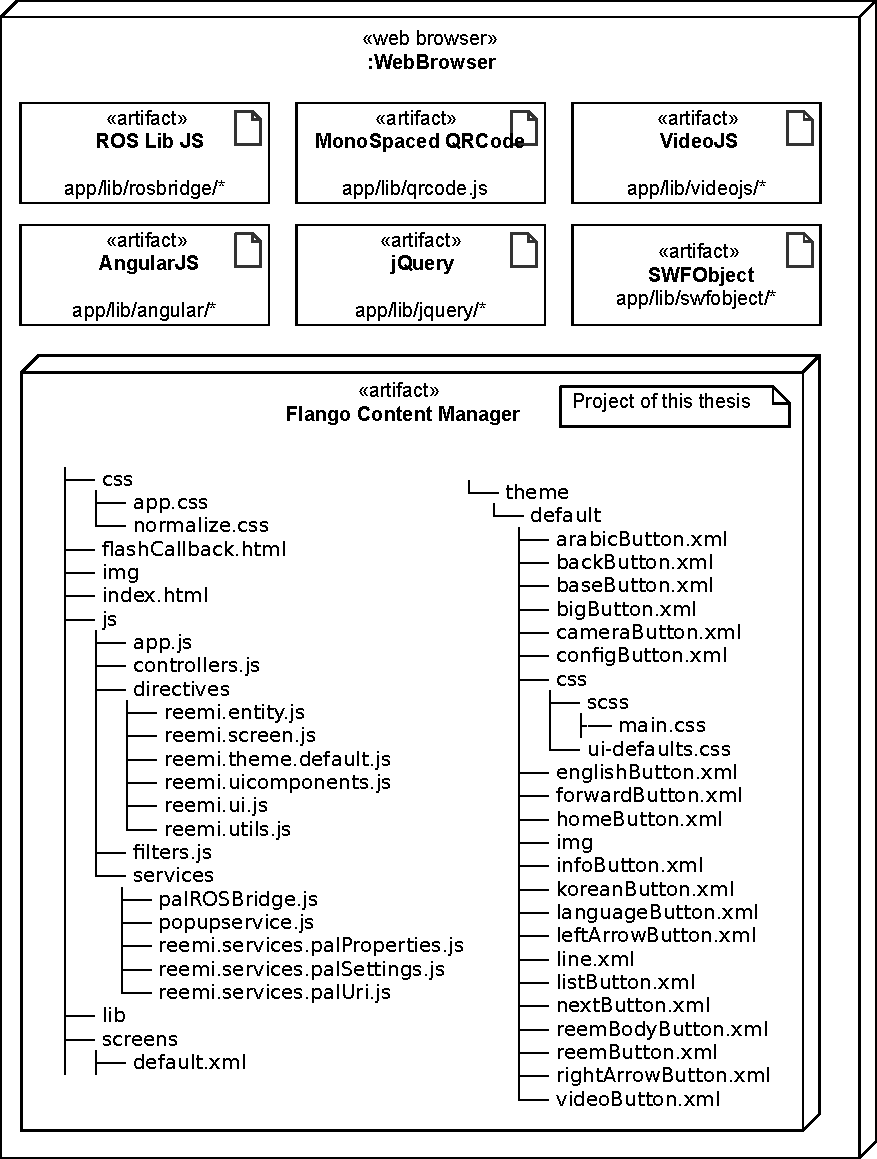
\includegraphics{figures/design-deployment-browser.pdf}
    \caption{Deployment Diagram: Browser}
    \label{fig:deploy-browser}
\end{figure}

\begin{figure}[htb]
    \centering
    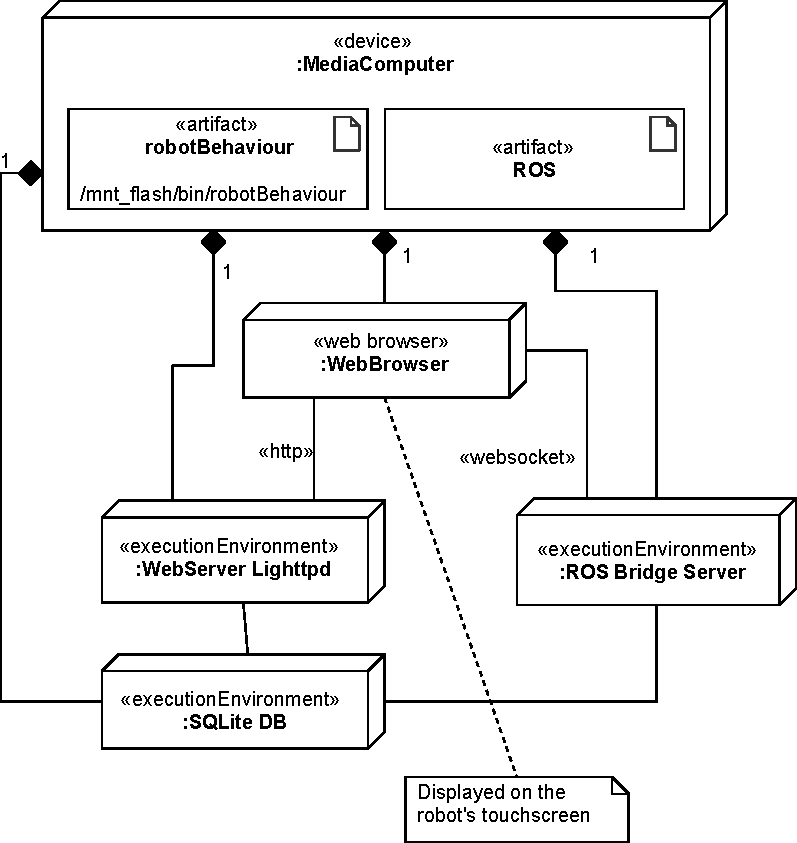
\includegraphics{figures/design-deployment-mediacomputer.pdf}
    \caption{Deployment Diagram: Media computer}
    \label{fig:deploy-media}
\end{figure}

\begin{figure}[htb]
    \centering
    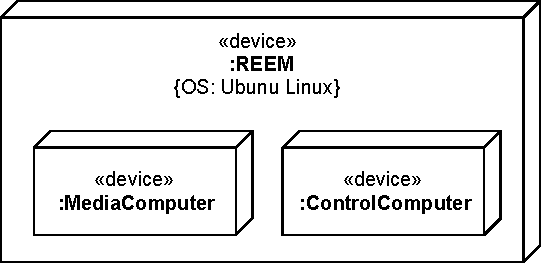
\includegraphics{figures/design-deployment-reem.pdf}
    \caption{Deployment Diagram: Reem}
    \label{fig:deploy-reem}
\end{figure}

\begin{figure}[htb]
    \centering
    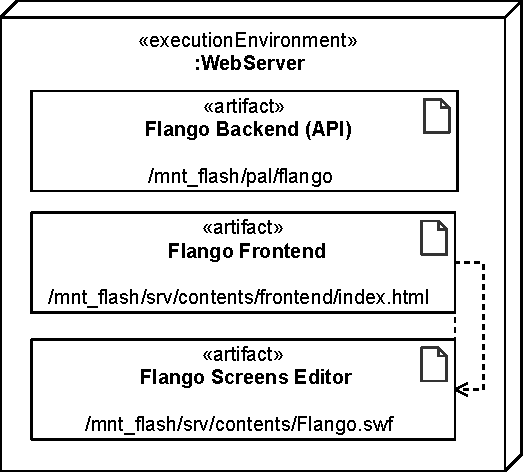
\includegraphics{figures/design-deployment-webserver.pdf}
    \caption{Deployment Diagram: Webserver}
    \label{fig:deploy-webserver}
\end{figure}

\FloatBarrier
